\clearpage
\refstepcounter{sourcechapter}
\phantomsection
\section*{附录 III\quad 20 世纪后半叶 Navier--Stokes 方程的若干进展}
\label{app:twentieth-century-developments}
\addcontentsline{toc}{section}{附录 III\quad 20 世纪后半叶 Navier--Stokes 方程的若干进展}
\setcounter{section}{0}
\setcounter{equation}{0}
\renewcommand{\theequation}{\arabic{equation}}
\MBSetSourceChapterAnchor{appendix-03}

\hypertarget{appendix-03-page-352}{}
\subsection*{引言}
\addcontentsline{toc}{subsection}{引言}

Navier--Stokes 方程(NSE)理论是当代数学物理的一个核心问题. 这些方程是描述许多常见现象的, 在物理上得到充分接受的模型. 流体力学工程师, 气象学家, 数学家以及其他研究者为此投入了大量工作, 但许多问题仍处在科学前沿. 从物理观点看, 一些表述极其简单的问题仍未解决, 例如确定湍流的热性质, 或描述湍流施加在其边界(如飞机或管道)上的力. 在数学方面, NSE 是研究非线性现象和非线性方程的模型, 而该领域本身尚处于早期阶段. NSE 及相关 Euler 方程包含非线性方程的四个核心问题: 适定性, 振荡, 间断和非线性动力学.

NSE 的数学理论技术性很强, 尽管仍不完整, 其内容已经十分庞大. 因此, 一篇讨论如此广泛主题的文章应当包含什么并不显然: 是描述结果而不成为结果目录, 是梳理技术与思想的演变, 还是讨论与湍流及物理学的联系. 本文未能令人满意地处理所有这些问题. 无疑存在许多重要遗漏, 许多重要主题也未获得足够篇幅; 本文作出了一些取舍, 而该领域的其他研究者很可能会作出不同选择. 大量参考文献在一定程度上弥补了这些不足. 尽管如此, 仍希望这些札记能对部分读者有用; 作者本人也在写作中学到了新内容, 并修正或巩固了已有认识.

本文把不可压缩流和可压缩流的方程都称为 Navier--Stokes 方程, 尽管有些作者只把不可压缩流方程称为 NSE. 两种情形都会讨论, 但重点放在数学理论更为成熟的不可压缩流.

NSE 的数学理论始于 J. Leray (1933,\allowbreak 1934a,b)的开创性工作. 他在分布理论由 L. Schwartz (1950, 1951)发展出来之前, 首次引入偏微分方程弱形式的概念; 在稍早时候, S.L. Sobolev (1936)系统引入了以其名字命名的空间.\footnote{正如 AMS Chelsea 版前言所述, 本附录 III 最初作为独立文章发表于 J. P. Pier (2000)主编的著作中. 经 Birkhauser 同意在此重印. 与本书其余部分一样, 本文版权属于 American Mathematical Society.}

\hypertarget{appendix-03-page-353}{}
J. Leray 奠定了我们今天所知的不可压缩 NSE 数学理论基础, 并引入了许多此后一直使用的工具和思想. 事实上, 尽管人们付出了大量努力, 自 J. Leray 的工作以来进展仍相对缓慢. Peter Lax 撰写的关于 Jean Leray 对偏微分方程理论(包括 NSE)贡献的精彩介绍, 收入了 Jean Leray 文集(1998).

与 Leray 同期但相互独立的工作, 是 Gunther, Lichtenstein 和 Wolibner 关于 Euler 方程的研究, 它们在很久以后才重新受到关注. 我们不知道 20 世纪 30 和 40 年代还有其他严格结果. 不过, Lamb, Prandtl, G.I. Taylor, von Karman 等人得到了重要的经验性和启发性结果. 20 世纪 40 年代, A.N. Kolmogorov (1941)发表了关于湍流的奠基性工作, J. von Neumann 及其合作者则在计算和气象学方面开创了新的研究活动. 在本文所考察时期的开端, E. Hopf (1951)的著名论文恢复了用现代泛函分析研究 NSE 的理论工作, 此后这一研究贯穿整个 20 世纪后半叶. 可压缩流的数学理论则在这一时期末发展起来.

本文将强调数学理论的两个方面: 一是在不可压缩情形中各种函数空间内解的适定性, 即存在性, 唯一性和正则性; 二是与湍流的联系, 尤其是 NSE 数学理论同 Kolmogorov 和 Kraichnan 传统湍流理论的联系. 还将以不同详细程度讨论其他主题, 包括可压缩 NSE, Euler 方程, 最优控制, 以及流体力学与其他现象耦合所产生的相关方程. 本文基本或完全未涉及的主题包括: 与分岔有关的向湍流转捩, NSE 与动力学理论的关系, NSE 与 $k-\epsilon$ 模型等湍流模型的关系, 非 Newton 流, 多流体和数值逼近. 如前所述, NSE 数值求解问题由 von Neumann 及其合作者在 20 世纪 40 年代开创. 随着近几十年计算机能力大幅提高, 数值模拟已发展为独立学科---计算流体力学, 位于工程学与物理学的交界处; 尽管如此, 这一学科仍提出具有重要数学内涵的问题.

作者感谢所有帮助准备本文的人, 特别是 David Hoff, Antonin Novotny 和 Denis Serre 对可压缩流一节的帮助, Ioana Moise 使用 American Mathematical Society 数据库协助书目检索, 以及所有阅读并评论本文早期版本的人.

本文结构如下:
\begin{itemize}
\item 第一部分: 不可压缩 Navier--Stokes 方程;
\item 第 \ref{sec:app3-existence} 节: 解的存在性, 唯一性和正则性;
\item 第 \ref{sec:app3-attractors} 节: 吸引子与湍流;
\item 第二部分: 其他问题, 其他方程;
\item 第 \ref{sec:app3-compressible-inviscid} 节: 可压缩流与无黏流;
\item 第 \ref{sec:app3-other-problems} 节: 若干其他问题与方程.
\end{itemize}

\hypertarget{appendix-03-page-354}{}
\begin{center}\textbf{第一部分: 不可压缩 Navier--Stokes 方程}\end{center}

\section{解的存在性, 唯一性和正则性}
\label{sec:app3-existence}

\paragraph{Navier--Stokes 方程.}
先简要回顾 Navier--Stokes 方程(NSE)的推导. 考虑一种流体, 它在时刻 $t$ 占据空间 $\mathbb R^3$ 中的区域 $\Omega_t$. 假设 $\Omega_t=\Omega$ 与时间无关, 因为运动区域的数学困难往往会掩盖 NSE 本身特有的困难. 在流体力学中, 运动的 Lagrange 表示给出每个流体质点的轨迹 $x=\Phi(a,t)$, 其中 $a$ 是质点在时刻 $0$ 的位置, $x$ 是时刻 $t$ 的位置. NSE 最常见的形式对应于流动的 Euler 表示, 它给出向量场 $u=u(x,t)$, 即时刻 $t$ 位于 $x$ 的流体质点的速度. 记
\[
x=(x_1,x_2,x_3),
\quad a=(a_1,a_2,a_3),
\quad u=(u_1,u_2,u_3).
\]
有
\[
u(x,t)=\frac{\partial\Phi}{\partial t}(a,t).
\]
反过来, 可由 Euler 表示通过求解常微分方程组 $x_a(t)=\Phi(a,t)$ 恢复 Lagrange 表示:
\begin{equation}
\frac{dx_a(t)}{dt}=u(x_a(t),t),
\qquad x_a(0)=a.
\label{eq:app3-particle-trajectory}
\end{equation}

动量守恒方程为
\[
\rho\gamma_i=f_i+\sigma_{ij,j},
\]
其中 $\rho=\rho(x,t)$ 是密度, $\gamma=\gamma(x,t)$ 是加速度, $f=f(x,t)$ 表示施加于流体的外部体力, $\sigma=(\sigma_{ij}(x,t))_{ij}$ 是 Cauchy 应力张量. 这里采用重复指标求和的 Einstein 约定, 并记 $\varphi_{,j}=\partial\varphi/\partial x_j$. 由运动学的链式求导,
\[
\gamma_i=\frac{\partial u_i}{\partial t}+u_ju_{i,j}.
\]
另一方面, 对所谓 Newton 流体, Cauchy 应力张量取为
\[
\sigma_{ij}=2\mu D_{ij}(u)+\lambda\operatorname{div}u\,\delta_{ij}-p\delta_{ij},
\qquad
D_{ij}(u)=\frac12(u_{i,j}+u_{j,i}),
\]
其中 $p=p(x,t)$ 是压力, $\mu>0$, $\lambda\in\mathbb R$. 因而一般 NSE 为
\begin{equation}
\rho\left(\frac{\partial u_i}{\partial t}+u_ju_{i,j}\right)
-\mu\Delta u_i-(\lambda+\mu)(\operatorname{div}u)_{,i}+p_{,i}=f_i.
\label{eq:app3-general-nse}
\end{equation}
另一个基本方程表示质量守恒(连续性方程):
\begin{equation}
\frac{\partial\rho}{\partial t}+\operatorname{div}(\rho u)=0.
\label{eq:app3-continuity}
\end{equation}
若流体不可压缩, 任一部分的体积在运动中保持不变, 即
\begin{equation}
\operatorname{div}u=0.
\label{eq:app3-incompressibility}
\end{equation}

\hypertarget{appendix-03-page-355}{}
此时质量守恒方程意味着 $\rho$ 沿流体轨迹为常数. 若流体还均匀, 则 $\rho(x,0)=\rho_0>0$ 与 $x$ 无关. 将 
\eqref{eq:app3-general-nse} 除以 $\rho_0$, 得到不可压缩均匀流的 NSE, 即 
\eqref{eq:app3-incompressibility} 以及
\begin{equation}
\frac{\partial u_i}{\partial t}+u_ju_{i,j}-\nu\Delta u_i+p_{,i}=f_i,
\label{eq:app3-incompressible-nse-components}
\end{equation}
或向量形式
\[
\frac{\partial u}{\partial t}+(u\cdot\nabla)u-\nu\Delta u+\nabla p=f.
\]
这里 $\nu=\mu/\rho_0$ 是运动黏度, 并把 $p/\rho_0,f/\rho_0$ 重新记为 $p,f$. 不可压缩非均匀流的方程由 
\eqref{eq:app3-general-nse}--\eqref{eq:app3-incompressibility} 组成, 其中 
\eqref{eq:app3-general-nse}, 
\eqref{eq:app3-continuity} 可利用 
\eqref{eq:app3-incompressibility} 化简. 在这些方程中均有黏性, $\mu,\nu>0$; 当 $\mu=\nu=0$ 时对应无黏或``理想''流体, 此时恢复 Euler 方程.

第一部分余下内容讨论 
\eqref{eq:app3-incompressibility}, 
\eqref{eq:app3-incompressible-nse-components} 以及在物理和(或)数学上有意义的简化形式, 即稳态流($u,p$ 与 $t$ 无关)和去掉二次项的线性化方程. Navier--Stokes 方程的一个显著性质是: 它们是数学物理中极少数(甚至可能是唯一的)非线性方程之一, 其非线性由数学论证(仅为链式求导)导出, 而非来自物理建模.

\paragraph{边界条件和初始条件.}
用边界条件和初始条件补充 
\eqref{eq:app3-incompressibility}, 
\eqref{eq:app3-incompressible-nse-components}. 假设 $\Omega$ 是 $\mathbb R^3$ 中具有 $C^r$ 边界 $\Gamma$ 的有界开集, $\Omega$ 局部位于 $\Gamma$ 的一侧, 至少 $r\geq2$. Dirichlet(或无滑移)边界条件
\begin{equation}
u=0\quad\text{在 }\Gamma\text{ 上}
\label{eq:app3-no-slip-boundary}
\end{equation}
(或给定 $u(x,t)=g(x,t)$)对应于边界 $\Gamma$ 是静止(或以指定速度 $g$ 运动)的实体边界. 另一个具有数学意义的情形是空间周期情形:
\begin{equation*}
u,p\text{ 在 }x_i\text{ 方向以 }L_i\text{ 为周期},
\qquad i=1,2,3.
\tag{6'}
\label{eq:app3-periodic-boundary}
\end{equation*}
此时 $\Omega=\prod_{i=1}^3(0,L_i)$ 是周期单元, 还指定 $\int_\Omega u=\int_\Omega f=0$. 这种流动当然不能在物理上直接实现, 但空间周期流对研究均匀湍流很有意义. 
\eqref{eq:app3-no-slip-boundary} 与 
\eqref{eq:app3-periodic-boundary} 的另一个物理差异是: 当 $\nu$ 很小时, 条件 
\eqref{eq:app3-no-slip-boundary} 会在 $\Gamma$ 附近产生边界层; 对空气, 水等常见流体正是如此. 从数学观点及目前的理论认识看, 在适定性和长时间行为方面, 两种边界条件差异不大. 不过 
\eqref{eq:app3-no-slip-boundary} 会带来一些现已充分理解的泛函分析困难; 在空间周期情形中, 使用 Fourier 级数即可容易解决.

\hypertarget{appendix-03-page-356}{}
本文不着重讨论的其他边界条件包括: $\Omega$ 无界; 通道流(两个方向周期, 第三个方向取 Dirichlet 条件); 以及液体水平表面等处的``自由边界''条件, 它给出 Neumann 型条件
\[
u\cdot n=0,
\qquad(\sigma\cdot n)_\tau=0
\quad\text{在 }\Gamma\text{ 上},
\]
其中 $n=(n_1,n_2,n_3)$ 是 $\Gamma$ 的外单位法向量, $(\sigma\cdot n)_\tau$ 是 $\sigma\cdot n$ 的切向分量, $\sigma$ 为 Cauchy 应力张量. 由于 
\eqref{eq:app3-incompressibility}, 后一条件化为
\[
n\times\operatorname{curl}u=0
\quad\text{在 }\Gamma\text{ 上}.
\]
还用速度初值补充方程:
\begin{equation}
u(x,0)=u_0(x)\quad(\text{给定}),
\qquad x\in\Omega.
\label{eq:app3-initial-velocity}
\end{equation}

未知函数 $u,p$ 的作用很不相同. 这可由边初值问题 
\eqref{eq:app3-incompressibility}--\eqref{eq:app3-initial-velocity} 的 Leray 弱形式看出; 也可直接看到, 在包括 $t=0$ 的每个时刻, $p$ 都是 $u$ 的函数, 由一个 Neumann 问题的解表示. 对方程 
\eqref{eq:app3-incompressible-nse-components} 的向量形式取散度, 得
\begin{equation}
\Delta p=\operatorname{div}f-u_{j,i}u_{i,j}.
\label{eq:app3-pressure-poisson}
\end{equation}
在空间周期情形 
\eqref{eq:app3-periodic-boundary} 中, 该方程由 $u,f$ 确定 $p$. 在条件 
\eqref{eq:app3-no-slip-boundary} 下, 再将动量方程与 $n$ 作内积, 得相应的 Neumann 边界条件
\begin{equation}
\frac{\partial p}{\partial n}=f\cdot n+\nu\Delta u\cdot n
\quad\text{在 }\Gamma\text{ 上}.
\label{eq:app3-pressure-neumann}
\end{equation}

\paragraph{函数空间与 Stokes 问题.}
以下集中讨论 
\eqref{eq:app3-no-slip-boundary}; 对 
\eqref{eq:app3-periodic-boundary} 的修改很容易, 而且后文大多数内容在该情形更直接. 在 $L^2$ 空间理论中, 考虑测试函数空间
\[
\mathcal V=\{v\in C_0^\infty(\Omega)^d:\operatorname{div}v=0\},
\]
并以 $H,V$ 分别表示 $\mathcal V$ 在 $L^2(\Omega)^d,H_0^1(\Omega)^d$ 中的闭包. 这里 $d$ 是空间维数, 本节所有结果均可推广到 $\Omega\subset\mathbb R^d$ 的情形. Sobolev 空间 $H^m(\Omega)$ 是 $L^2(\Omega)$ 中分布导数直到 $m$ 阶均属于 $L^2(\Omega)$ 的函数空间; $H_0^1(\Omega)$ 是 $H^1(\Omega)$ 中在 $\Gamma$ 上消失的函数子空间. 由 Poincaré 不等式, $H_0^1(\Omega)^d$ 与 $V$ 对内积和范数
\[
((u,v))=\sum_{j=1}^d\left(\frac{\partial u}{\partial x_j},\frac{\partial v}{\partial x_j}\right),
\qquad
\lVert u\rVert=((u,u))^{1/2}
\]
均为 Hilbert 空间, 其中
\[
(f,g)=\int_\Omega f(x)g(x)\,dx,
\qquad |f|=(f,f)^{1/2}.
\]

\hypertarget{appendix-03-page-357}{}
这里 $u,v,f,g$ 可为标量或向量; $H$ 对范数 $|\cdot|$ 当然也是 Hilbert 空间. $H,V$ 可刻画为
\[
H=\{v\in L^2(\Omega)^d:\operatorname{div}v=0, v\cdot n|_{\partial\Omega}=0\},
\]
\[
V=\{v\in H_0^1(\Omega)^d:\operatorname{div}v=0\}.
\]
$H$ 与 $\Omega$ 的第一上同调空间之间关系的进一步性质见 Foias and Temam (1978).

Stokes 问题是 
\eqref{eq:app3-incompressibility}, 
\eqref{eq:app3-incompressible-nse-components}, 
\eqref{eq:app3-no-slip-boundary} (或 
\eqref{eq:app3-periodic-boundary})的稳态线性化形式; 取 $\nu=1$ 即
\begin{equation}
\left\{
\begin{aligned}
-\Delta u+\operatorname{grad}p&=f&&\text{在 }\Omega\text{ 中},\\
\operatorname{div}u&=0&&\text{在 }\Omega\text{ 中},\\
u&=0&&\text{在 }\Gamma\text{ 上}.
\end{aligned}
\right.
\label{eq:app3-stokes-problem}
\end{equation}
在空间周期情形中, 可用 Fourier 级数容易求解. 在 Dirichlet 情形中, 由下述弱形式和 Riesz 表示定理(或投影定理)立刻得到 $u$ 的存在唯一性. 更困难的是 Stokes 问题的正则性理论. Cattabriga (1961)和 Solonnikov (1964, 1966)利用 Agmon, Douglis and Nirenberg (1959, 1964)的椭圆系统正则性理论方法, 在 $L^2,L^p$ 空间中发展了这一理论. $L^2$ 空间中较简单的证明见 Ghidaglia (1986). 若 $f\in H^m(\Omega)^d$, $m\geq-1$, 则 $u\in H^{m+2}(\Omega)^3$, $p\in H^{m+1}(\Omega)$, 且 $u,p$ 线性连续依赖于 $f$; 这里假设 $\Gamma$ 为 $C^r$ 类, $r\geq m+2$.

令 $D(A)=V\cap H^2(\Omega)^d$, 对 $u\in D(A)$ 定义 $Au=-P\Delta u$, 其中 $P$ 是 $L^2(\Omega)^d$ 到 $H$ 的正交投影(本文建议称为 Leray--Helmholtz 投影). 由上述正则性结果, $A$ 是从 $D(A)$ 到 $H$ 的同构; 其逆 $A^{-1}$ 在 $H$ 中自伴, 正且紧, 并有 $H$ 中完整的规范正交特征向量基:
\[
Aw_j=\lambda_jw_j,
\qquad j\geq1,
\qquad \lambda_j\to\infty\quad(j\to\infty).
\]
Metivier (1978)给出了 $j\to\infty$ 时 $\lambda_j$ 的行为: $\lambda_j\sim c j^{2/d}$, 其中 $d$ 是空间维数, 此处为 $3$; 它与 Laplace 算子的特征值相同(见 Courant and Hilbert (1953)). 还可定义 $A$ 的幂 $A^s$, $s\in\mathbb R$, 其定义域为 $D(A^s)$; $A^r$ 是从 $D(A^{s+r})$ 到 $D(A^s)$ 的同构.

最后简述 Stokes 问题的弱形式. 以 $v\in\mathcal V$(或 $V$)乘 
\eqref{eq:app3-stokes-problem} 第一式并在 $\Omega$ 上积分, 得
\[
u\in V,
\qquad ((u,v))=(f,v),
\quad\forall v\in V.
\]
由 Riesz 定理得到 $u$ 的存在唯一性. 恢复 $p$ 则使用对 $\operatorname{grad}\mathcal D'(\Omega)$ 的下述刻画, 其中 $\mathcal D'(\Omega)$ 是 $\Omega$ 上的分布空间:
\begin{equation}
M\in\operatorname{grad}\mathcal D'(\Omega)
\quad\Longleftrightarrow\quad
\langle M,\varphi\rangle=0,
\quad\forall\varphi\in\mathcal V.
\label{eq:app3-gradient-distribution-characterization}
\end{equation}
该刻画可由 De Rham 流理论推出. L. Tartar (1976)给出的较简单证明使用了 J.L. Lions 在 Magenes and Stampacchia (1958)中对 $L^2(\Omega)$ 的刻画: 它是满足 $\operatorname{grad}\varphi\in H^{-1}(\Omega)^d$ 的分布 $\varphi$ 所成的空间, 其中 $H^{-1}(\Omega)$ 是 $H_0^1(\Omega)$ 的对偶. X. Wang (1993)还给出了 
\eqref{eq:app3-gradient-distribution-characterization} 的一个简单自足证明.

\hypertarget{appendix-03-page-358}{}
\paragraph{弱形式, 存在性与唯一性结果.}
J. Leray 引入的 Navier--Stokes 方程弱形式, 是以测试函数 $v\in\mathcal V$(或 $V$)乘动量方程并在 $\Omega$ 上积分所得. 以 $u(t)$ 表示函数 $x\in\Omega\mapsto u(x,t)$. 寻求几乎处处 $t>0$ 时属于 $V$ 的 $u(t)$, 使下式在 $(0,T)$ 或 $(0,\infty)$ 上的分布意义成立:
\begin{equation}
\frac d{dt}(u(t),v)+\nu((u(t),v))+b(u(t),u(t),v)=(f(t),v),
\quad\forall v\in V,
\qquad u(0)=u_0.
\label{eq:app3-weak-nse}
\end{equation}
在相应积分有定义时,
\[
b(u,v,w)=\sum_{i,j=1}^d\int_\Omega u_i\frac{\partial v_j}{\partial x_i}w_j\,dx.
\]

在 $L^2$ 理论中, 通常把 
\eqref{eq:app3-weak-nse} 中属于 $L^2(0,T;V)\cap L^\infty(0,T;H)$, 对每个 $T>0$, 的解称为弱解; 把属于 $L^2(0,T;D(A))\cap L^\infty(0,T;V)$ 的解称为强解. 存在唯一性结果随空间维数而异. 解的存在性通常由构造法得到: 例如用 Galerkin 方法或时间和(或)空间有限差分构造近似解, 再利用解的先验估计取极限. 也可用 Leray--Schauder 不动点定理, 或简单的 Banach 不动点定理, 后者通常只在``小''时间区间 $0<t<T_*$ 上产生解. 任何证明的关键似乎都是建立先验估计; 它们依赖于对 $b$ 的估计. 这类估计很多, 通常结合 Hölder 不等式与 Sobolev, Agmon, Ladyzhenskaya, Gagliardo--Nirenberg 或插值不等式得到.

Leray 对全空间二维情形(1933)证明了解在所有时间的存在唯一性, 对二维有界区域(1934a)证明了解在依赖于数据的区间 $(0,T_*)$ 上的存在唯一性. 他还研究了三维全空间情形(1934b), 证明正则解在某个依赖数据的区间 $(0,T_*)$ 上存在唯一, 并证明弱解在所有时间存在, 同时讨论了奇性可能出现的问题. Hopf (1951)证明了三维有界区域, 边界速度为零时弱解在所有时间的存在性. Hopf 使用与 Leray 相同的框架, 但以 Galerkin 方法构造近似解; Leray 则通过磨光非线性项得到近似方程并构造近似解. 下一个基本结果是 Lions and Prodi (1958)证明的二维弱解唯一性. 大约同时, Ladyzhenskaya (1958, 1959)改进了 Leray 关于二维有界区域强解的存在性结果; 加上后来证明的结果, 特别是 Stokes 方程和稳态 Navier--Stokes 方程的正则性, 它获得了最终形式.

J. Leray 把 NSE 的弱解称为湍流解. 他引入弱解概念的动机之一, 是考虑一类允许 curl 向量变为无穷的解, 以描述湍流. 他提出的三维湍流中奇性是否可能出现的问题至今未解决: 三维 NSE 中奇性的存在既未被证明, 也未被否证.

\hypertarget{appendix-03-page-359}{}
概括而言, 在 $L^2$ 空间框架下, 存在唯一性理论的状况如下:
\begin{itemize}
\item 当 $d=2$ 时, 理论相当令人满意. 问题在 Hadamard 意义下适定: 弱解存在唯一; 数据适当正则时强解存在唯一; 更一般地, 只要数据 $u_0,f,\Omega$ 足够正则, 解具有数据所允许的全部正则性, 包括 $C^\infty$ 正则性和解析性; 并且在相应函数空间中连续依赖于数据.
\item 当 $d=3$ 时, 只有部分结果: 强解在依赖数据的区间 $(0,T_*)$ 上存在唯一; 弱解在 $(0,+\infty)$ 上存在. 弱解唯一性以及强解在所有时间存在性仍是公开问题. 与二维一样, 强解只要存在, 就具有数据所允许的光滑性, 直至 $C^\infty$ 正则性和解析性. 实际上不存在``中间层次''的正则性: 一旦弱解例如属于 $L^6(0,T;V)$ 或 $L^\infty(\Omega\times(0,T))^3$, 它就是强解, 并具有数据允许的光滑性.
\end{itemize}

\MBSourceStatementNumber{remark}{1}
\begin{Remark}
\label{rem:app3-classical-l2-theory}
上述结果现已构成 NSE 经典 $L^2$ 理论的核心. 除前述原始论文外, 可见 Ladyzhenskaya (1969), J.L. Lions (1969), Constantin and Foias (1988), Temam (1984, 1995)等著作, 后者强调周期情形. Marion and Temam (1997)列出了一份很长但仍不穷尽的相关结果清单. P.L. Lions (1996)的近著包含经典结果和许多新结果.
\end{Remark}

三维情形已有若干部分结果. Leray (1933)证明, 无外力($f=0$)时 NSE 的所有解最终都会光滑, 即在某个依赖数据的 $T_*>0$ 之后光滑. Serrin (1963)证明, 若强解在 $(0,T)$ 上存在, 则 $(0,T)$ 上不存在其他弱解. Foias, Guillopé and Temam (1981)以及 Duff (1989, 1990, 1991)证明弱解属于 $L^{2/3}(0,T;D(A))$, 还属于其他空间 $L^q(0,T;H^m(\Omega)^d)$, 其中 $0<q<1$, $m>2$.

下面还将回顾一些关于奇性可能出现或解爆破的结果. 先评论 Kato and Fujita (1962)一个不太为人熟知的结果: 若 $f$ 在某种意义下很小, 且 $u_0$ 在 $H^{1/2}(\Omega)^3$ 中很小, 则三维 Navier--Stokes 方程的光滑解在所有时间存在. 稍作不同表述并为简单起见取 $f=0$, 证明基于在 
\eqref{eq:app3-weak-nse} 中以 $A^{1/2}u(t)$ 代替 $v$ 所得的能量型方程. 适当估计非线性项后得到
\[
\frac12\frac d{dt}|A^{1/4}u|^2+\nu|A^{3/4}u|^2
=-b(u,u,A^{1/2}u)
\leq c_1|A^{1/4}u||A^{3/4}u|^2.
\]
若 $|A^{1/4}u_0|\sim|u_0|_{H^{1/2}}<\nu/c_1$, 则 $|A^{1/4}u(t)|$ 对所有 $t>0$ 递减. 在 
\eqref{eq:app3-weak-nse} 中以 $Au(t)$ 代替 $v$ 得到的类似关系又意味着 $H^1$ 范数也衰减:

\hypertarget{appendix-03-page-360}{}
\[
\frac12\frac d{dt}\lVert u\rVert^2+\nu|Au|^2
\leq c_1|A^{1/4}u||Au|^2.
\]
若 $u_0$ 集中在高频上, 即 $u_0=\sum_{j=J}^\infty u_{0j}w_j$, $J$ 很大, 则
\[
\lVert u_0\rVert\geq\lambda_J^{1/4}|A^{1/4}u_0|.
\]
由此可知, 当 $u_0,f$ 高度振荡时, 即使 $\lVert u_0\rVert$(以及类似的 $|f|$)任意大, 三维 NSE 的解仍在所有时间存在且光滑. Cannone and Meyer (1995)在 Besov 空间框架中证明了给出类似结论的深刻结果; 另见 Bondarevsky (1996)的公告和下文 Furioli, Lemarié--Rieusset and Terraneo (1997)的结果. 这清楚表明, 三维 NSE 强解的存在性不仅依赖于 $u_0,f$ 的大小, 还依赖于它们的高频分量; 因而需要使用能够反映数据和解的谱性质的方法或函数空间.

\MBSourceStatementNumber{remark}{2}
\begin{Remark}
\label{rem:app3-singularity-physical-scale}
这里不猜测三维 NSE 是否会出现奇性, 即 $\lVert u(t)\rVert$ 是否会在有限时间变为无穷. 但应注意, 这意味着在比碰撞平均自由程甚至原子直径更小的短波长处仍存在``大量活动''; 例如集中在这些波长上的旋量总量 $\lVert u(t)\rVert^2=|\operatorname{curl}u(t)|_{L^2(\Omega)}^2$ 将为无穷. 于是必须把这一事实与 Navier--Stokes 方程的物理基础协调起来, 后者用动力学理论的流体动力学极限定义 $\nu$. 同样的评论不适用于 Euler 方程.
\end{Remark}

\paragraph{其他结果与其他空间($L^p,C^\infty,C^\omega$, Hardy).}
在 $L^2$ 空间框架中, Fujita and Kato (1964)使用了半群理论; 另见 Henry (1981), von Wahl (1985), Pazy (1983), 以及较近的 Ben Artzi (1994), Brezis (1994). 上文着重讨论有界区域, 但对演化方程而言, 大多数结果很容易推广到无界情形. 此外, 关于无界稳态区域, 尤其是外部区域(紧光滑集的补集), 还有大量独立文献. 这里的问题包括 $|x|\to\infty$ 时 $u(x)$ 的衰减性质, 以及由能量关系确定的自然空间
\[
\{u\in\mathcal D'(\Omega)^d:\partial u_i/\partial x_j\in L^2(\Omega),\ i,j=1,\ldots,d\}
\]
不再是 $H^1(\Omega)$. 特别见 Finn (1959a,b, 1961, 1965a,b)和 Heywood (1972, 1974a,b, 1976)的论文, 后者还研究了无界区域空间 $V$ 的一个出人意料的性质. Babin and Vishik (1990), Babin (1992)等研究了带权 Sobolev 空间在无界区域稳态和非稳态 Navier--Stokes 方程中的使用. M. Schonbek (1991, 1992, 1995, 1996)在一系列论文中研究全空间 $\mathbb R^2$ 或 $\mathbb R^3$ 中 NSE 及相关方程解在 $t\to\infty$ 时的衰减, 对大数据解得到最优代数衰减率; 衰减分析的主要思想是 Fourier 分裂法.

许多作者研究了 Stokes 和 Navier--Stokes 方程的自由边界值问题, 例如 Abergel and Bona (1992), Beale (1981, 1984), Solonnikov (1977, 1982).

\hypertarget{appendix-03-page-361}{}
NSE 的 $L^p$ 理论包括大量关于 $L^p(L^p)$ 或 $L^p(L^q)$ 空间中存在性和(或)唯一性的结果, 其中 $L^p(L^q)=L^p(0,T;L^q(\Omega)^d)$. 在所考察时期始终有相关结果, 很早的工作包括 Serrin (1959, 1962, 1963)和 Prodi (1959). Solonnikov (1964, 1968)建立了线性演化 Stokes 问题的存在性与正则性理论, 即动量方程去掉 $(u\cdot\nabla)u$; 由此可借助插值与逐步提升法推导许多 NSE 结果, 也就是把 $(u\cdot\nabla)u$ 看作源项. von Wahl (1985)的著作以及许多论文着重讨论 $L^p$ 理论. 虽然一些 $L^p$ 结果可由 $L^2$ 理论特别是 Solonnikov 的工作恢复, 许多结果要求完全不同的方法, 并要求从向量场 Helmholtz--Leray 分解 $L^2(\Omega)^d=H\oplus H^\perp$ 的类似物开始, 重新思考和处理理论的多个方面. Furioli, Lemarié--Rieusset and Terraneo (1997)证明了 Kato 温和解 $u\in C([0,\infty);L^3(\mathbb R^3))$ 的唯一性, 假设 $u_0$ 在 $L^3(\mathbb R^3)$ 中的范数很小.

Serre (1983)研究了分片正则区域(角和拐角)中 Stokes 或 Navier--Stokes 方程解的 $L^2,L^p$ 正则性; Fabes, Kenig and Verchota (1988), Shen (1991), Brown and Shen (1995)等研究了 Lipschitz 区域. 对分片 $C^2$ 光滑区域, 另见 Osborn (1976)和 Grisvard (1985).

回到光滑区域. 强解的 $C^\infty$ 正则性可由 $L^2$ 理论及 $\Omega$ 为 $C^\infty$ 时 $\bigcap_{m=1}^\infty H^m(\Omega)=C^\infty(\overline\Omega)$ 推出; 见 Guillopé (1982, 1983)及 Marion and Temam (1997)中的其他陈述. Masuda (1967)证明了解的空间解析性. Iooss (1973)证明了取值于 $D(A)$ 或其他空间的时间解析性, Foias and Temam (1979)以不同方法也证明了这一点. Foias and Temam (1989)证明了空间周期情形中 Gevrey 类的空间正则性; 相关结果见 Henshaw, Kreiss and Reyna (1990). Grubb, Solonnikov and Geymonat 在一系列论文中用伪微分算子研究 Stokes 和 Navier--Stokes 方程, 例如 Grubb and Solonnikov (1992), Grubb (1995), Grubb and Geymonat (1977, 1979).

Coifman, Lions, Meyer and Semmes (1993)利用补偿紧性(Tartar (1979))研究惯性非线性项 $(u\cdot\nabla)u$ 在 Hardy 空间中的行为, 并得到 Hardy 和 $L^1$ 空间中的正则性结果. Cannone and Meyer (1995)(另见 Cannone (1995))利用 Littlewood--Paley 分解, 研究 $\mathbb R^2$ 或 $\mathbb R^3$ 中 Besov 及其他空间内解的存在性.

所有这些函数空间中的结果都与 $L^2$ 空间中的结果相似: 解在小时间区间存在唯一; 当 $d=2$ 时可能在所有时间存在, 当 $d=3$ 时则在某些条件下如此. 各种函数空间方法并非彼此无关; 相反, 它们相互联系并彼此受益.

NSE 解在 $t\to0$ 时的行为与正则性是一个偏微分方程问题, 它在热方程或演化 Stokes 线性方程中已经出现. 对有界区域, 例如边界条件 
\eqref{eq:app3-no-slip-boundary} 而非 
\eqref{eq:app3-periodic-boundary}, 除非数据 $u_0,f$ 满足某些相容性条件, 正则解的高阶 Sobolev 范数 $H^m(\Omega)$, $m\geq3$, 会在 $t=0+$ 附近爆破. 与热方程等不同, 由于压力作用, 这些相容性条件在空间上是全局的. Iooss (1970)用半群理论研究了该问题, 另见 Heywood (1979), Heywood and Walsh (1994), Temam (1982). 这种奇异行为可能影响有界区域中方程的数值解, 例如 Gresho (1990).

\hypertarget{appendix-03-page-362}{}
Bardos and Tartar (1973)及 Ladyzhenskaya (1975)证明了 NSE 的反向唯一性: 若 $u=u_1$ 和 $u=u_2$ 是 
\eqref{eq:app3-weak-nse} 第一式在所有 $t<0$ 上的正则解, 且 $u_1(0)=u_2(0)$, 则对所有 $t<0$ 都有 $u_1(t)=u_2(t)$.

三维 NSE 适定性的其他部分结果包括: Fursikov (1980)证明, 对稠密集 $L^p(0,T;V')$ 中的每个 $f$, 任意 $1<p<4/3$, 三维 NSE 适定, 即强解对所有 $t>0$ 存在. 另有一系列结果表明, 对三维薄区域 $\Omega=\Omega_\epsilon=\omega\times(0,\epsilon)$, $\omega\subset\mathbb R^2$, $0<\epsilon<\epsilon_0$, 在适当的 $\epsilon_0$ 及某类``大数据'' $u_0,f$ 下, 三维 NSE 适定; 见 Raugel and Sell (1992, 1993), Temam and Ziane (1996). Temam and Ziane (1997)还在与地球物理流研究有关的球形区域 $a<r<a+\epsilon$ 中得到类似结果.

最后简述 $d\geq4$ 的空间维数. 对非线性演化方程(完整 NSE), 结果稍弱但本质上与三维情形相似, 例如 Lions (1969). 对非线性稳态情形, Frehse and Ruzicka (1994a,b)和 Struwe (1997)研究了解的正则性; 其中使用了 Serrin (1959)观察到的事实: 对稳态 NSE, $\frac12|u|^2+p$ 满足极大值原理.

\paragraph{奇性, 自相似性与爆破.}
考虑三维 NSE 
\eqref{eq:app3-weak-nse} 的弱解 $u$, 假设 $f,u_0$ 光滑, 至少 $f\in L^2(0,T;H)$, $u_0\in V$. 若 $u\in L^6(0,T;V)$ 或 $u\in L^\infty(\Omega\times(0,T))^3$, 则 $u$ 是强解. 因而若存在不是强解的弱解, 即出现奇性, 则 $\lVert u(t)\rVert=|\operatorname{curl}u(t)|_{L^2(\Omega)^3}$ 会在有限时间变为无穷, 或 $|u|_{L^\infty(\Omega\times(0,T))}=+\infty$.

Leray 在其开创性工作中研究了奇性可能出现的问题, 并指出集合 $\{t\in[0,T]:\lVert u(t)\rVert=+\infty\}$ 的 Lebesgue 测度为零, 甚至在 $[0,T]$ 中具有零的 $1/2$-Hausdorff 维数; 该集合在 $[0,T]$ 中的补集是可数个半闭区间 $[a_i,b_i)$ 之并. Scheffer (1977)首次研究时空奇异集的大小. 随后 Caffarelli, Kohn and Nirenberg (1982)证明, 奇异集 $\{(x,t)\in\Omega\times(0,T):|u(x,t)|=+\infty\}$ 的一维 Hausdorff 测度为零. 特别地, 奇性不能位于光滑曲线上, 至多位于一个``更小的集合''上. Fang-Hua Lin and Chun Liu (1997)以及 Gang Tian and Zhouping Xin (1997)最近给出了 Caffarelli, Kohn and Nirenberg 结果的简化推导.

Leray 还指出, 若三维 NSE 的正则解在 $[0,T)$ 上于 $T$ 变为奇异, 则当 $t\to T-0$ 时, $\lVert u(t)\rVert$ 至少以 $\operatorname{const}/\sqrt{T-t}$ 的速度爆破. 迄今尚未发现这样的解. Leray 提出可能存在如下形式的奇异自相似解:
\begin{equation}
u(x,t)=\frac1{\sqrt{2a(T-t)}}
U\left(\frac{x}{\sqrt{2a(T-t)}}\right),
\label{eq:app3-singular-self-similar}
\end{equation}
其中 $a>0$. 他证明, 若 $U\not\equiv0$ 是 $\mathbb R_y^3$ 中方程组
\begin{equation}
-\nu\Delta U+aU+a(y\cdot\nabla)U+(U\cdot\nabla)U+\nabla P=0,
\qquad\operatorname{div}U=0
\label{eq:app3-self-similar-profile}
\end{equation}
的解,

\hypertarget{appendix-03-page-363}{}
并且 $U$ 的某些范数有限, 特别是 $U\in L^\infty(\mathbb R_y^3)\cap L^2(\mathbb R_y^3)$ (Leray 1934, p. 225), 则 
\eqref{eq:app3-singular-self-similar} 中的 $u$ 在 $t=T-0$ 产生奇性. Nečas, Růžička and Šverák (1996)最近证明, 
\eqref{eq:app3-self-similar-profile} 属于 $L^3(\mathbb R_y^3)$ 的唯一解是 $U\equiv0$. 与稳态 Navier--Stokes 方程一样, $\frac12|U|^2+P$ 满足极大值原理, 这被用于证明 
\eqref{eq:app3-self-similar-profile} 不存在非零解. Tai-Peng Tsai (1997)更近一步证明, 除恒等于零外, 不存在局部能量和局部旋量均有限的相似解. 因而这些结果排除了 
\eqref{eq:app3-singular-self-similar} 型物理可接受奇性的存在.

出于完全不同的动机, Cannone and Meyer (1995), Cannone (1995)研究 $\mathbb R^3\times(0,\infty)$ 中 NSE 自相似解的存在性, 其形式为 
\eqref{eq:app3-singular-self-similar}, 但把 $T-t$ 替换为 $t$. 他们把问题表述为初值问题, 初值是 $-1$ 次齐次函数, 并在 $u_0$ 在适当空间中很小时求解该初值问题. 近年来还广泛研究了其他非线性方程的自相似解, 例如 Giga and Kohn (1985), Souplet and Weissler (1997).

\section{吸引子与湍流}
\label{sec:app3-attractors}
\setcounter{equation}{14}

本节讨论 NSE 与湍流关系的若干方面. 这本身又是一个广阔主题, 本节绝不是对相关文献的全面描述. 特别地, 不讨论与稳定性和分岔理论有关的向湍流转捩问题, 而集中讨论湍流的永久状态和充分发展湍流.

把 NSE 与湍流联系起来的首次尝试来自 Leray. 他猜测 NSE 会出现奇性, 并引入湍流解概念. A.N. Kolmogorov 的工作和传统湍流理论则以现象学概念为基础, 实际很少使用 NSE. 下文所述当前研究背后的数学计划是: 我们能从 NSE 中了解到哪些湍流性质? 对这一问题的一些有限贡献, 一方面严格证明传统湍流理论中某些公认且可赋予数学内容的事实, 另一方面构造适合或看来适合进一步发展这种联系的数学工具.

湍流的数学描述主要有两条途径. 它们并非完全无关, 而且都与 NSE 有关:
\begin{enumerate}
\item 传统湍流理论以统计描述为基础. 数学上的自然对象是在函数空间 $H$ 上定义, 并按 Navier--Stokes 方程随时间演化的测度.
\item 动力系统方法. 沿着动力系统理论的发展以及 S. Smale, D. Ruelle and F. Takens 的思想, 湍流的永久状态与包含解的全部长时间行为的全局吸引子相联系.
\end{enumerate}

\hypertarget{appendix-03-page-364}{}
\paragraph{NSE 的统计解.}
传统湍流理论通常考虑 NSE 的统计解, 其中对快速振荡的物理量作时间和(或)空间平均, 并显式或隐式引入相应测度 $\mu$. 与数学方法较接近的资料包括 Batchelor (1970), Onsager (1949), Orszag (1972), Monin and Yaglom (1971), Frisch (1995), 另见 Foias, Manley, Rosa and Temam (2000)即将出版的著作.

在数学文献中, Foias and Prodi 发展了 NSE 统计解的数学概念, 见 Foias (1973)的长篇论文. 由 NSE 控制的 $H$ 上概率测度 $\mu_t$ 的演化由 Hopf 方程(1951)给出. 它是 Liouville 方程的 Fourier 变换:
\[
\frac d{dt}\int_H\Phi(u)\,d\mu_t(u)
+\int_H\{((u,\Phi'(u)))+b(u,u,\Phi'(u))-(f,\Phi'(u))\}\,d\mu_t(u)=0,
\]
其中 $\Phi$ 遍及适当的测试泛函类, 使 $\Phi'(u)\in V$. 上述文献对这一方程证明了与 Leray 三维 NSE 理论类似的存在唯一性定理. 利用泛函 Fourier 变换, 也对 Hopf 方程证明了类似结果. 这些结果适用于有界区域或周期情形. Vishik and Fursikov (1977a,b, 1980)处理了与物理上重要的均匀湍流相适应的均匀流情形, 即空间平移不变测度, 并研究了测度各阶矩之间的关系. 随后 Foias and Temam (1980, 1983), Foias, Manley and Temam (1988)寻找自相似统计解; 它们的存在性与 Leray 方程 
\eqref{eq:app3-self-similar-profile} 的一个变形有关, 其中 $a(y\cdot\nabla)U$ 替换为 $-a(y\cdot\nabla)U$.

\paragraph{平稳统计解.}
时间无关的统计解很重要, 因为它们与遍历性和吸引子有关. 特别地, 已证明如下存在性与逼近结果: 若 $u$ 是 NSE 
\eqref{eq:app3-incompressible-nse-components}, 边界条件 
\eqref{eq:app3-no-slip-boundary} 或 
\eqref{eq:app3-periodic-boundary}, 以及初值 
\eqref{eq:app3-initial-velocity} 的解, 且 $f$ 与时间无关, 则 $u$ 的时间平均
\begin{equation}
\frac1T\int_0^T u(\cdot,t)\,dt
\label{eq:app3-time-average-velocity}
\end{equation}
在 $T\to\infty$ 时``收敛''到 NSE 的平稳统计解 $\mu=\mu_f$. 流体力学中猜测遍历性成立, 并认为时间平均与空间平均收敛到同一极限, 因而该极限唯一确定. 从数学观点看, 平均的收敛对某些子序列 $T'\to\infty$ 成立, 或在 Banach 极限 $\operatorname{LIM}$ 的弱意义下成立, 见 Dunford and Schwartz (1958)以及 Foias and Temam (1980), Bercovici, Constantin, Foias and Manley (1995)中的应用. 典型地, 对任意从 $H$ 到 $\mathbb R$ 的弱连续函数 $\Phi$,
\begin{equation}
\operatorname{LIM}_{T\to\infty}\frac1T\int_0^T\Phi(u(t))\,dt
=\int\Phi(u)\,d\mu_f(u).
\label{eq:app3-banach-limit-statistical-solution}
\end{equation}

\hypertarget{appendix-03-page-365}{}
在二维情形, 测度 $\mu_f$ 在与 
\eqref{eq:app3-incompressible-nse-components}, 
\eqref{eq:app3-no-slip-boundary}--\eqref{eq:app3-periodic-boundary}, 
\eqref{eq:app3-initial-velocity} 相联系的半群 $\{S(t):u(0)\mapsto u(t)\}_{t\geq0}$ 下不变:
\[
\int\Phi(S(t)u)\,d\mu(u)=\int\Phi(u)\,d\mu(u),
\qquad\forall t\geq0.
\]
三维情形具有较弱形式的不变性. 该测度 $\mu$ 是 Hopf 方程的解, 后者是空间 $H$ 中具有无穷多个变量的微分方程. 上述文献还导出了平稳统计解 $\mu_f$ 的其他性质. 特别地, 这种测度由全局吸引子 $\mathcal A$ 承载, 即
\begin{equation}
\mu(H\setminus\mathcal A)=0.
\label{eq:app3-statistical-measure-attractor-support}
\end{equation}

\paragraph{随机 Navier--Stokes 方程.}
随机 NSE 也得到广泛研究, 虽然并不直接参照传统湍流理论. 特别是外力 $f$ 包含白噪声的情形, 见 Bensoussan and Temam (1973), Viot (1976), Da Prato and Zabczyk (1996). 另见 Flandoli and Gatarek (1995)与 Flandoli and Maslowski (1995)的较新论文. 前者考虑相当一般的白噪声, 寻找鞅解或概率意义下的平稳解; 后者研究加性噪声下不变测度的唯一性与遍历性. Avellaneda and Majda (1991, 1992, 1994)通过研究随机输运方程, 得到了与湍流理论有关的精确结果.

\paragraph{吸引子.}
湍流的永久状态与 NSE 解的长时间行为有关. 在湍流的动力系统方法中, 关注方程的全局吸引子, 它包含在固定且与时间无关的外力 $f$ 下, 所有初值 $u_0$ 所产生解的全部长时间行为. 除了由无穷维动力系统一般定理推出全局吸引子的存在性外, 主要贡献还包括: 证明吸引子具有有限维数; 给出维数上下界; 并给出具有物理意义的吸引子维数上界, 即与传统湍流理论的相关估计一致.

NSE 所生成的动力系统及吸引子的存在性见 Ladyzhenskaya (1973, 1975). Foias and Temam (1979)证明二维 NSE 的全局吸引子具有有限 Hausdorff 维数和分形维数. 对三维情形, 任意在 $V$ 中有界的函数不变集 $X$, 即 $S(t)X=X$ 对所有 $t\geq0$, 也有同样结论. 后一论文中, 吸引子 $\mathcal A$ 的维数关于 Reynolds 数或 Grashof 数呈指数型, 其中
\[
Gr=|f|\nu^{-2}L^{3-d/2},
\]
$L$ 是 $\Omega$ 的一个典型长度. 此后, Babin and Vishik (1983a, 1983b, 1985, 1986), Constantin and Foias (1985), Constantin, Foias and Temam (1985, 1988), Ladyzhenskaya (1985, 1987), Lieb (1984), Ruelle (1982/83), Temam (1986)隐式或显式使用 Lyapunov 指数, 得到关于 $Re$ 或 $Gr$ 的多项式界. Temam (1986)对二维, 边界条件 
\eqref{eq:app3-no-slip-boundary} 且 $Gr$ 很大时给出 $\dim\mathcal A\leq cGr$. Constantin, Foias and Temam (1988)对二维, 边界条件 
\eqref{eq:app3-periodic-boundary} 给出
\[
\dim\mathcal A\leq cGr^{2/3}(\log Gr)^{1/3},
\]
且该界近乎最优: Liu (1994)证明此时 $\dim\mathcal A\geq cGr^{2/3}$.

\hypertarget{appendix-03-page-366}{}
Babin and Vishik (1985, 1986)首次给出 NSE 全局吸引子维数的下界. 他们考虑狭长区域 $(0,1)\times(0,L)$ 中的二维空间周期流, 对大 $L$ 得到 $\dim\mathcal A\geq cL$. Ziane (1997)改进 Constantin, Foias and Temam (1985)的一般结果, 在此情形得到最优上界 $\dim\mathcal A\leq c'L$, 与 Babin and Vishik 的下界吻合.

吸引子维数估计的物理意义来自下面讨论的湍流有限维性概念. 关于 NSE 吸引子的更完整讨论, 可见 Babin and Vishik (1992), Hale (1988), Ladyzhenskaya (1991), Temam (1997)等著作及其中参考文献.

二维全局吸引子或三维中在 $V$ 内有界的函数不变集, 是完整轨道 $\{u(t)\}_{t\in\mathbb R}$ 之并, 这些轨道在所有时间上满足 
\eqref{eq:app3-weak-nse} 第一式. Foias and Temam (1979)表明, 这些轨道关于时间在复时间平面的带状区域 $|\operatorname{Im}\tau|<\delta$ 内解析, 而带宽 $\delta$ 对吸引子上的所有轨道统一有效. $\delta$ 的数值似乎具有物理意义, Foias 及其合作者在多篇论文中研究了它, 例如 Foias (1997). 我们希望了解吸引子以及吸引子上流动动力学的更多信息, 但遗憾的是, 除上述结果外所知甚少.

\paragraph{湍流的有限维性.}
在永久状态中, 湍流显示有限维性. Landau and Lifschitz (1953)的著作把它描述为``湍流的有限自由度数''. 为简单起见考虑空间周期情形 
\eqref{eq:app3-periodic-boundary}. 在三维中, 由 Kolmogorov 定律, 能谱(对统计平均)
\[
E(k)=\frac12\sum_{\substack{j\in\mathbb Z^d\\|j|\geq k}}|\widehat u_j|^2,
\qquad
u=\sum_{j\in\mathbb Z^d}\widehat u_je^{ij\cdot x},
\]
在 $k>k_d$ 时很小并呈指数衰减. 这里 $k_d$ 是 Kolmogorov 耗散波数, 其量级为 $k_0Re^{3/4}$, $k_0$ 是一个典型宏观波数. 因而所有活跃模在统计意义上包含于球 $|j|\leq k_d$ 中, 可容易数出 $(k_d/k_0)^3$ 个活跃模. Constantin, Foias, Manley and Temam (1985)以及 Constantin, Foias and Temam (1985)用适当的 $k_d$ 定义, 以 $c(k_d/k_0)^3$ 估计吸引子维数. 二维情形有类似结果, 界为 $c(k_\eta/k_0)^2$, 其中 $k_\eta$ 是 Kraichnan 耗散波数.

还引入并研究了其他流动有限维性概念. Foias and Prodi (1967)首次引入决定模概念: 若 $f(t)=f$, $u_1,u_2$ 是 
\eqref{eq:app3-weak-nse} 分别以 $u_{01},u_{02}$ 为初值的两个解, $P_N$ 是适当的有限维投影, 且
\[
P_N(u_1(t)-u_2(t))\to0\quad(t\to\infty),
\]
则
\[
u_1(t)-u_2(t)\to0\quad(t\to\infty).
\]

\hypertarget{appendix-03-page-367}{}
Foias, Manley, Temam and Treve (1983)扩展了决定模概念. Foias and Temam (1984)引入决定结点概念, Jones and Titi (1992)证明了与吸引子维数估计相当的决定结点数估计. Foias and Temam (1979)提出的轨道压缩性质是流动有限维性的另一个有用概念. 所有这些有限维性概念都为``湍流的有限自由度数''这一物理概念赋予了数学意义和严格证明.

最后, 惯性流形(IM)概念是流动有限维性的另一形式. 已对包括超黏性 NSE 在内的许多耗散方程证明 IM 的存在性, 其中以 $\epsilon(-\Delta)^r$ 代替 $-\nu\Delta$, 但尚未对 NSE 本身证明; 见 Foias, Sell and Temam (1985, 1988). Kwak (1993)宣布了 NSE 本身惯性形式的存在性, 但证明并不完整.

惯性流形存在时, 它是一个有限维光滑流形, 所有轨道都以指数速度收敛到它. 其方程形如 $z=\Phi(y)$, 其中 $z=(I-P_N)u$, $y=P_Nu$, $P_N$ 是适当的有限维投影; 它给出高模由低模支配的规律. 如前所述, NSE 惯性流形是否存在仍是公开问题, 但已经得到多种近似惯性流形, 例如 Foias, Jolly, Kevrekidis, Sell and Titi (1988), Foias, Manley and Temam (1987, 1988), 以及 Temam (1997)列出的其他文献.

\paragraph{NSE 与湍流的其他联系.}
传统湍流理论普遍认为, 时间平均能量耗散率与黏度无关. Doering and Constantin (1992, 1995)考虑通道流, 导出了与 Kolmogorov 标度一致的能量耗散率上界. X. Wang (1997)把结果推广到更一般的边界驱动流. 这里一个关键技术工具是把 $\Omega$ 的边界 $\Gamma$ 上定义的函数适当延拓到区域内部; X. Wang 的构造改进了 Hopf 的经典构造. 空间周期情形见 Foias (1997).

Bercovici, Constantin, Foias and Manley (1995)进一步研究了 NSE 吸引子与相应统计解之间的关系. 如前所述, 初值位于全局吸引子上的二维 NSE 解具有全局时间解析性. 解析区域是复时间域中宽度为 $\delta$ 的带状区域, 其中 $\delta$ 与轨道无关, 并且是 Grashof 数的递减函数. Bercovici, Constantin, Foias and Manley (1995)证明, 因此频谱, 即空间一点处湍流速度双时间相关的 Fourier 变换 $P(\omega)$, 其中 $P(\omega)$ 为正测度, 在高频处至少以 $\exp(-\delta|\omega|)$ 的速度衰减. 这里对频谱给出了严格定义, 避免了关于包含二维 NSE 湍流解的相空间具有度量不可分解性的通常假设.

\hypertarget{appendix-03-page-368}{}
\begin{center}\textbf{第二部分: 其他问题, 其他方程}\end{center}

\section{可压缩流与无黏流}
\label{sec:app3-compressible-inviscid}
\setcounter{equation}{17}

\subsection*{可压缩黏性流}

\paragraph{演化方程.}
如前所述, 可压缩 Navier--Stokes 方程(CNSE)是 
\eqref{eq:app3-general-nse}, 
\eqref{eq:app3-continuity}. 它们出现在非稀薄可压缩流体高 Mach 数流动的应用中. 应区分可压缩流体与可压缩流动: 可压缩流体的低 Mach 数流动密度几乎为常数, 因而可合理地用不可压缩 Navier--Stokes 方程(INSE)描述. 可压缩情形中压力的作用也与不可压缩情形大不相同. 在后一情形, $p$ 是 $u$ 的函数, 通过 Neumann 问题 
\eqref{eq:app3-pressure-poisson}, 
\eqref{eq:app3-pressure-neumann} 求得; 在 INSE 的大部分数学理论中压力先消失, 最后再恢复. 可压缩情形中压力是独立函数. 仅数 
\eqref{eq:app3-general-nse}, 
\eqref{eq:app3-continuity} 的方程和未知量, 就会看到还需要一个方程. 对正压流, 补充流体状态方程 $P=P(\rho)$. 对非正压流, 状态方程形如 $P=g(\rho,e)$, $e$ 是流体内能; 此时再以表达能量守恒即热力学第一定律的能量方程补充 
\eqref{eq:app3-general-nse}, 
\eqref{eq:app3-continuity}. 本文只考虑正压流及相应 CNSE.

CNSE 的许多数学问题当然与 INSE 相同: 存在性, 唯一性, 连续依赖性和长时间行为. 但关注重点有两个重要差异. 在 CNSE 应用中, 压力远大于其他力, 因而黏性项和对流项较不重要. 这意味着很大一部分数学分析用于逐点或至少在适当范数中控制密度与压力, 而 INSE 中没有这一问题. 另一个相关方面是, 解的重要定性特征在很大程度上与黏度无关; 人们希望借助相应无黏 Euler 方程的典型结构理解 CNSE 解, 包括激波, 剪切波, 稀疏波或压缩波和接触间断.

存在唯一性定理从 Kanel (1968), Kazhikov and Shelukhin (1977)等人的一维理论开始; 不同于 INSE, 一维理论并非平凡. 他们的分析采用非标准能量方法, 从局部时间解的总熵随时间不减这一观察出发. Matsumura and Nishida 从 1979 年开始的一系列论文把该方法推广到二维和三维. 分析的技术性强得多, 更多依赖于正确预测相应线性化方程的渐近衰减率. 他们对小而光滑的初值证明了接近常状态的小光滑解的整体存在性.

较新的结果放宽了对初值的限制. Lions (1993)以及 Kazhikov and Weigant (1995)用更现代的弱紧性技术, 在某些正压流 $P=P(\rho)$ 情形对大初值获得整体解. Hoff (1995)深入分析完整非正压 CNSE 中初始间断的影响,

\hypertarget{appendix-03-page-369}{}
发现奇性随流输运并随时间指数衰减; 黏度越小, 声速越大, 衰减越快. 这种效应是底层无黏 Euler 方程双曲性的结果, 因而是上述观点的一个实例.

上述工作中外力并不起重要作用. 可压缩 Euler 方程解与 CNSE 解之间的关系十分重要, 目前已有大量研究投入其中. 迄今结果仅限于一维. 例如 Tai-Ping Liu and Yanni Zeng (1997)证明``黏性激波''具有动力稳定性; 它是一维 CNSE 的行波解, 具有无黏激波的物理特征. 这是首个表明无黏可压缩 Euler 方程的典型结构对 CNSE 解具有重要意义的结果.

\paragraph{稳态方程.}
控制方程是去掉时间导数的 
\eqref{eq:app3-general-nse}, 
\eqref{eq:app3-continuity}. 热力学第二定律要求 $\mu>0$, $3\lambda+2\mu\geq0$, 演化情形也如此. 假设 $p=g(\rho)$, 通常为 $p=k\rho$ 或 $p=k\rho^\gamma$, $\gamma>1$. 若 $p$ 还依赖温度, 则必须引入热方程或能量方程, 本文不讨论.

稳态问题通常在 $\mathbb R^d$ 的光滑有界区域 $\Omega$ 中考虑, 外部情形则在这种区域的补集中考虑. 在 $\partial\Omega$ 上指定 $u=u_*$, 大多数论文取 $u_*\cdot n=0$; 外部情形还要求 $u\to u_\infty$, $\rho(x)\to1$ 当 $|x|\to\infty$. 已得到两类结果:
\begin{enumerate}
\item 平衡态 $\rho_0=1$, $u_*=u_\infty$ 附近强解的存在唯一性, 内部情形默认 $u_\infty=0$. 对未知量 $\sigma=p-1$, $v=u-u_\infty$ 得到混合椭圆--双曲系统, 再用不动点法及以下方法之一求解:
  \begin{itemize}
  \item 对系统作椭圆正则化并用 Matsumura and Nishida (1983)引入的特殊技术作局部估计; 见 Farwig (1989), Padula (1987), Pileczas and Zajaczkowski (1990), Valli (1987).
  \item 对向量场作 Leray--Helmholtz 分解 $v=w+\nabla\varphi$, $\operatorname{div}w=0$, 并写出诱导方程; 见 Novotny (1994, 1997)的一系列结果及其他待发表论文.
  \end{itemize}
\item 弱解的存在性. P.L. Lions (1993a,b)首先证明了一系列结果, 包括等熵情形弱解 $(\rho,u)\in L^q(\Omega)\times W_0^{1,2}(\Omega)$ 的存在性, 其中 $1<q(\gamma)<+\infty$, 条件为 $d=2$ 时 $\gamma>1$, $d=3$ 时 $\gamma\geq5/3$. 例如 $\Omega$ 为有界区域并取上述边界条件. 他还证明了解的部分正则性: $\rho\in L_{\mathrm{loc}}^\infty(\Omega)$, $u\in W_{\mathrm{loc}}^{1,s}(\Omega)$ 对每个 $1<s<+\infty$, 且
\[
\Pi=k\rho^\gamma-(2\mu_1+\mu_2)\operatorname{div}u
\in W_{\mathrm{loc}}^{1,2}(\Omega)
\]
对 $d=2$, $\gamma>1$, 或 $d=3$, $\gamma>3$ 成立. 证明依赖连续性方程的重整化解概念, 并重写动量方程以出现交换子
\[
\rho v_i\partial_i(-\Delta)^{-1}\partial_j(\rho v_j)
-\partial_i(-\Delta)^{-1}\partial_j(\rho v_iv_j).
\]
关键是用 Coifman, Lions, Meyer and Semmes (1993)的结果获得该项的弱紧性.
\end{enumerate}

\hypertarget{appendix-03-page-370}{}
Novotny (1996)讨论了弱解框架下 Helmholtz 分解的使用及 Hardy 空间 div--curl 引理的应用. 如引言所述, CNSE 理论比 INSE 理论更近, 但近年来发展迅速, 而且问题和困难也不同. P.L. Lions 关于 INSE 的近著之后, 第二卷专论 CNSE, 已刚刚出版.

\subsection*{Euler 方程}

本段简述与 Euler 方程有关, 足以单独成文的一些结果和问题. 读者可在 Majda (1984), Chemin (1995), P.L. Lions (1996)及其中参考文献中找到大量进展和讨论.

Euler 方程描述无黏流体, 也称``无黏''或``理想''流体. 在 
\eqref{eq:app3-general-nse} 中令 $\lambda=\mu=0$, 或在 
\eqref{eq:app3-incompressible-nse-components} 中令 $\nu=0$.\footnote{下文还简述黏度趋于零, 即 $\mu$ 或 $\nu\to0$, 的问题.} 此时 Cauchy 应力张量为球张量 $\sigma_{ij}=-p\delta_{ij}$. 流体仍可压缩或不可压缩; 后者又可均匀或非均匀. 本文着重讨论均匀不可压缩流, 不讨论不可压缩非均匀流, 对可压缩无黏流也只作极简叙述. 事实上, 后一情形的 Euler 方程数学理论更接近守恒律方程理论, 而不是 NSE 理论.

\paragraph{不可压缩流.}
在不可压缩均匀情形, Euler 方程是 
\eqref{eq:app3-incompressible-nse-components} 的向量形式和 
\eqref{eq:app3-incompressibility}, 其中 $\nu=0$. 初边值问题按 
\eqref{eq:app3-initial-velocity} 指定 $u$ 的初值, 边界条件可取 
\eqref{eq:app3-periodic-boundary} 的空间周期性; 或者以不可穿透条件代替 
\eqref{eq:app3-no-slip-boundary}:
\begin{equation}
u\cdot n=0
\quad\text{在 }\Gamma\text{ 上}.
\label{eq:app3-euler-nonpenetration}
\end{equation}
压力仍是辅助变量, 在每个时刻通过 Neumann 问题 
\eqref{eq:app3-pressure-poisson}, 
\eqref{eq:app3-pressure-neumann} 由 $u$ 表示, 但 
\eqref{eq:app3-pressure-neumann} 中 $\nu=0$. 这显著改变了 $p$ 对 $u$ 的函数依赖关系, 可用于证明解的存在性. 另一种选择是采用类似于 
\eqref{eq:app3-weak-nse} 的变分形式, 令 $\nu=0$, 并例如要求 $v\in H\cap H^1(\Omega)^d$; 因而惯性非线性项成为方程的本质项.

对 
\eqref{eq:app3-incompressible-nse-components} 的向量形式施加 curl 算子, 可写出涡量 $\omega=\operatorname{curl}u$ 的方程:
\begin{equation}
\frac{\partial\omega}{\partial t}+(u\cdot\nabla)\omega
=(\omega\cdot\nabla)u+\operatorname{curl}f.
\label{eq:app3-vorticity-equation}
\end{equation}
当 $d=2$ 时 $\omega$ 为标量, 
\eqref{eq:app3-vorticity-equation} 右端的 $(\omega\cdot\nabla)u$ 消失; 因而 $f=0$ 时涡量沿流线守恒. $d=3$ 的情形显著不同.

关于动量方程在 $\nu=0$ 时, 配以 
\eqref{eq:app3-initial-velocity}, 
\eqref{eq:app3-euler-nonpenetration} (或 
\eqref{eq:app3-periodic-boundary}; 若 $\Omega=\mathbb R^d$ 则令 $u$ 在无穷远趋于零)的边值问题, 已知结果包括:

\hypertarget{appendix-03-page-371}{}
\begin{enumerate}
\item 在任意空间维数, 小时间区间上光滑解存在唯一. 更精确地, 令 $X_m=H\cap H^m(\Omega)^d$. 若 $u_0\in X_m$, $f\in L^\infty(0,T;X_m)$, $m-1>d/2$, 则对某个依赖 $u_0,f,\Omega$ 的 $T_*\leq T$, 解 $u$ 存在且属于 $C([0,T_*);X_m)$. 存在性证明基于先验估计
\begin{equation}
\frac d{dt}\lVert u\rVert_{H^m}
\leq c\bigl(\lVert u\rVert_{H^s}\lVert u\rVert_{H^m}+\lVert f\rVert_{H^m}\bigr),
\label{eq:app3-euler-apriori-estimate}
\end{equation}
它对任意 $s>1+d/2$ 成立, $c=c(s,\Omega)$.
\item 当 $d=2$ 时, 任意 $T>0$ 上光滑解存在唯一. 若给定 $u_0\in C^\alpha(\overline\Omega)$, $\operatorname{div}u_0=0$, $u_0\cdot n=0$ 在 $\partial\Omega$ 上, 且 $f\in C^{1+\alpha,0}(\overline\Omega\times[0,T])$, 则 Euler 方程的解存在唯一, 且 $u,p,\partial u/\partial x_i,\partial p/\partial x_i\in C(\overline\Omega\times[0,T])$; 通常 $p$ 在相差一个仅依赖 $t$ 的函数意义下唯一.
\item 当 $d=2$, $\Omega=\mathbb R^2$, $f=0$, 初始涡量 $\omega_0$ 是具有紧支集的有界符号测度, 且涡片 $\omega_0\in H^{-1}(\mathbb R^2)$ 时, 对任意 $T>0$ 都存在 Euler 方程的解 $u\in L^\infty(0,T;L_{\mathrm{loc}}^2(\mathbb R^2)^2)$.
\end{enumerate}

Euler 方程数学理论由 Lichtenstein (1930)和 Wolibner (1933)在二维情形开创. 第二项的证明见 Kato (1967). 第一项的全空间证明见 Kato (1972), 另见 Ebin and Marsden (1970), Bourguignon and Brezis (1974), Temam (1975), 后者由 Temam (1986)补全. 对有界 $\Omega$, Temam (1975)给出一个基于以 $u$ 估计 $p$ 的简短证明, 该估计可能在其他地方也有用. 第三项由 Delort (1991)证明; Schochet (1995)大幅简化了原证明, Majda (1993)改进了结果.

由 
\eqref{eq:app3-euler-apriori-estimate} 可知, 只要 $\lVert u(t)\rVert_{H^s}$ 有限, Euler 方程的解便保持光滑. Beale, Kato and Majda (1984)的更强结果只要求 $\operatorname{curl}u$ 在 $L^1(0,T_*;L^\infty(\Omega))$ 中的范数有界; Ponce (1985)只要求变形张量 $D_{ij}(u)$ 的空间最大范数关于时间可积.

只要解存在, 且 $u_0,f$ 足够正则, 就可得到 $H^m$ 直至 $C^\infty$ 的更高正则性. 与 Navier--Stokes 方程不同, 这里没有正则化效应: $u(\cdot,t)$ 与 $u_0(\cdot)$ 一样光滑, 不会更光滑.

Bardos, Benachour and Zerner (1976)证明 Euler 方程解关于时间在复时间平面适当区域内解析. 关于用 Besov 空间证明 Euler 方程解的存在唯一性, 见 M. Vishik (1997a,b).

Arnold (1972)在 Euler 方程背景下指出``似乎存在无穷多个不稳定构型''. 不稳定性问题与线性化 Euler 算子的谱结构密切相关; 不同于 Navier--Stokes 情形, 该算子不是椭圆的. Friedlander and Vishik (1991, 1992, 1993)构造了一种检测谱本质部分不稳定性的工具, 它基于可视为``流体 Lyapunov 指数''的几何量.

与 Navier--Stokes 方程一样, 一个重要问题是有限时间奇性是否可能出现. 问题仍未解决; 但 Euler 方程有一些部分结果, 而且证明奇性出现或获得奇性存在的``数值证据''(如 Kerr (1997))的尝试多于反方向的尝试.

\hypertarget{appendix-03-page-372}{}
Euler 方程理论还有一整部分研究非光滑解, 特别是涡斑, 即涡量为阶梯函数; 参考文献见 Constantin (1995)的综述. Chemin (1995)特别证明, 若 $\mathbb R^2$ 中初值是涡斑, 即在一个紧集上为常数, 且支集边界属于 $C^{1,\alpha}$, $0<\alpha<1$, 则解作为涡斑在所有时间存在, 且支集边界仍属于同一 $C^{1,\alpha}$ 类.

还应提到以测度为初值的 Navier--Stokes 或 Euler 方程. 多位作者研究了该问题, 例如 Cottet (1986), Giga, Miyakawa and Osada (1988), Michaux and Rakotoson (1993), Kato (1994), Constantin and Wu (1995). Ben-Artzi (1994)和 Brezis (1994)证明, 当 $f=0$ 且 NSE 初值属于 $L^1(\mathbb R^2)$, Euler 方程初值属于 $L^1(\mathbb R^2)\cap L^r(\mathbb R^2)$, $r>2$, 时, Navier--Stokes 与 Euler 方程的光滑解在所有时间存在唯一.

Euler 与 Navier--Stokes 方程的另一重要联系是 $\nu\to0$ 时 NSE 的行为. 只要 Euler 方程解光滑, 全空间或空间周期情形已经充分理解, 见 Kato (1984); 剩余问题是用 $\nu$ 表示收敛速度. 若相应 Euler 解不光滑, 即使在全空间; 或区域有边界, 即使相应 Euler 解光滑, NSE 解向 Euler 方程解收敛的问题\footnote{有些作者甚至认为 NSE 的解不收敛到相应 Euler 方程的解.}仍完全开放, 并且是数学物理的重大问题之一.

关于奇性的形成, DiPerna and Majda (1987)的奠基性工作揭示了可能发生现象的复杂性, 特别是会导致动能损失的集中和振荡, 这妨碍 Euler 方程存在性理论的发展. 对有界区域, 问题还包括在数学上未解决的湍流边界层. 最近出现了一些进展: Sammartino and Caflisch (1996)利用 Cauchy--Kowalewska 定理的抽象形式, 在解析解框架下证明半平面中完整 NSE 在小时间区间的收敛性; Sammartino (1996)还研究半平面中非稳态 Stokes 问题在黏度消失时的渐近行为. R. Temam and X. Wang (1997)对二维有界区域证明 NSE 解收敛到 Euler 方程解, 明确写出边界层函数, 并假设一个物理上合理的条件: 压力切向梯度在边界有界; 或当黏度趋于零时, 某个速度分量的切向导数在边界层中增长不太快. Kato (1984)在假设整个速度梯度增长不太快时证明了类似结果.

经典 Prandtl 方程被认为在一定程度上是边界层内 NSE 的有效逼近. Oleinik (1963)和 Fife (1967)研究了该方程. Weinan E and Engquist (1997)最近证明, 对某些紧支集数据, 非稳态 Prandtl 方程的光滑解会爆破.

\hypertarget{appendix-03-page-373}{}
\paragraph{可压缩流体.}
如前所述, 可压缩流 Euler 方程本质上属于守恒律方程理论. 它们与 NSE 的关系在于, 有些作者认为, 要推进可压缩 NSE 理论, 就需要充分理解全空间中 Euler 方程逼近 NSE 的方式.

简述若干结果; 截至 1972 年的完整叙述见 Lax (1973). 对正压和非正压情形, 小数据弱解的整体存在性由适用于一般守恒律的 Glimm 定理(1965)推出. Di Perna (1983a,b)首次把补偿紧性用于守恒律方程组, 研究正压流解的存在性. 沿着 Di Perna 的工作, Gui-Qiang Chen (1996, 1997)也用补偿紧性证明这类流动解的整体存在性, 初值和解可包含真空 $\rho=0$. Glimm and Lax (1970)的定理适用于正压流, 解与初值在 $L^\infty$ 中, 且 $t>0$ 时 $u(t)\in BV$, 即使 $t=0$ 时不成立; 但假设 $u_0$ 的振荡幅度很小. 另见 Nishida and Smoller (1973): 当 $P=\rho$ 时给出整体弱解; 当 $P=\rho^\gamma$, $\gamma>1$, 时对 $u_0$ 的全变差作出限制. Serre (1997), Grassin and Serre (1997)在适当假设下, 对任意空间维数得到在所有时间定义的光滑解.

\section{若干其他问题与方程}
\label{sec:app3-other-problems}

\paragraph{相关方程与近似方程.}
这里主要列出导致非常相似数学问题的一些相关方程, 以及通常会产生特定数学问题的一些近似方程.

当存在其他物理现象时, Navier--Stokes 或 Euler 方程可与其他方程耦合. 对导电流体, 例如等离子体, 海水或铝工业中的冰晶石, 存在电磁现象; 控制方程是 Maxwell 方程与 NSE 适当耦合所得的磁流体力学方程. 对热工水力学, NSE 与热方程耦合, 特别是在 Boussinesq 逼近中. 对燃烧或反应流, NSE 与热方程及复杂程度不等的化学方程耦合; 化学方程包括每种组分浓度的方程. 在所有这些情形中, 流体方程和其他方程可以有或没有黏性, 流体可以可压缩或不可压缩. 对不可压缩均匀 Newton 流体, 若所有方程都有黏性, 方程适定性理论与相应 NSE 单独存在时得到完全相同的结果; 极大值原理适用于温度和浓度.

对海洋, 大气, 河流等浅水问题, 引入了 NSE 的修正形式. 所谓浅水方程(法语文献中的 Saint-Venant 方程)提出完全不同的数学问题, 例如 Orenga (1995). 大气和海洋的所谓原始方程是气象学和海洋学的基本方程, 适用于高度相对地球半径很小的情形. 它们由带有 Coriolis 力的 NSE 构成, 水平速度满足动量守恒方程, 而在竖直方向, 动量守恒方程由静力方程代替; 还可与温度和湿度方程或盐度方程耦合. Lions, Temam and Wang (1992a,b, 1995)最近发展了这些方程的数学研究: 经过适当建模, 方程被写成与 NSE 泛函形式相似的形式, 但其非线性项更复杂, 结果也弱于三维不可压缩流体 NSE 的结果. 关于气候方程的其他一些数学问题, 见例如 Beale (1994), Embid and Majda (1996).

\hypertarget{appendix-03-page-374}{}
在另一种背景下, 也可考虑球面上带或不带 Coriolis 力的二维 NSE. 建立适当的几何框架后, 其适定性结果与二维 NSE 相同, 已相当完整; 对 Euler 方程见 Ebin and Marsden (1970), 另见 Ghidaglia (1986).

与 Euler 方程相关的另一主题是浅水中的波传播. 适当的渐近展开导出 Korteweg--de Vries 方程, 非线性 Schr\"odinger 方程或相关的水波方程. 这是与孤子有关的另一主题, 读者可参阅专门文献.

最后, NSE 基于 Newton 流的假设. 对非 Newton 流体, 可引入超黏性, 即以 $\varepsilon(-\Delta)^r$, $r>1$, 代替 $-\nu\Delta$, 见 Lions (1959, 1965); 或引入非线性黏性, 见 Ladyzhenskaya (1959). 关于非 Newton 流还有大量独立文献, 例如用于聚合物流动; 见 Joseph and Renardy (1993)及其中参考文献.

\paragraph{更具体的问题与定性性质.}
这里再提及 NSE 的若干其他方面, 它们会产生特定的问题和技术.

首先回顾前面已提到的不可压缩与可压缩流体在无界区域中稳态解的特殊问题. 对有界区域中的不可压缩流, 稳态解的非唯一性及其稳定性属于分岔理论, 其中会使用拓扑度理论等工具. 通常选取一个特征参数, 如 Reynolds 数或类似的数, 并研究参数变化时解的数目及其稳定性; 涉及两个或更多参数的分岔会变得非常复杂. 关于抽象分岔结果见 Rabinowitz (1973). 关于 NSE, 特别参见 Golubitsky, Iooss, Kirchgassner, Yudovich, Benjamin and Joseph 及其合作者的工作; 后两位还很好地结合了理论与实验. 另见 Iooss and Joseph (1980)以及讨论对称性影响的 Golubitsky and Schaeffer (1985).

如前所述, 对湍流, 即使数据与时间无关, 永久状态也可能依赖时间. 时间依赖性首次出现于 Hopf 分岔: 稳态解分岔为时间周期解, 相应永久状态是时间周期流. Hopf (1943)引入以他命名的分岔现象时, 其动机当然来自流体力学. 近来 Chenciner, Iooss 等人研究了 NSE 的 Hopf 分岔及其他分岔.

对 NSE 作适当无量纲化后, $\nu\simeq\mathrm{Re}^{-1}$, 其中 $\mathrm{Re}$ 为流动的 Reynolds 数. 物理上有意义的流动具有很大的 Reynolds 数, 例如普通或工业流动为 $10^4$ 至 $10^8$, 地球或其他行星上的地球物理流动为 $10^{12}$ 至 $10^{18}$.

\hypertarget{appendix-03-page-375}{}
当 Reynolds 数很大时, 对有壁流动, 在靠近壁面的薄区域中会出现尚未充分理解的重要物理现象. 该区域通常厚度为 $\mathrm{Re}^{-1/2}$, 称为边界层. 前面已经提到, 对有壁流动, 当 $\nu\to0$ 时 Navier--Stokes 方程是否收敛到 Euler 方程仍是开放问题; 困难当然与对边界层现象理解不足有关.

值得指出的是, 过去几十年的实验室研究使人们对 NSE 解的定性行为获得了一些认识, 这些研究曾经并且仍可帮助提出数学猜想. 例如物理学家 Libchaber 关于边界层和分岔的实验, H. Swinney 关于分岔和向混沌过渡的实验, 以及流体力学工程师 B. Benjamin and D. Joseph 关于分岔的实验; 如前所述, 后两位把理论与实验结合起来.

\paragraph{数值分析与计算流体力学.}
由于 NSE 极其复杂, 除了具有许多对称性的极特殊问题外, 不可能找到相应边值问题的精确解. 因此, 对物理或工程中任何实际感兴趣的问题, 只能希望通过数值模拟计算近似解. 机械工程界和数学界目前都投入了大量工作, 地球物理流体动力学方面的巨大努力更不必说. 目前, 对具有物理意义的流动还无法直接数值模拟 NSE 本身, 即所谓 Direct Numerical Simulation (DNS), 通常需要采用某种湍流模型, 如 $k$--$\varepsilon$ 模型, Large Eddy Simulation 和 Smagorinsky 模型. 对三维 DNS, 由常规湍流理论以及吸引子维数研究的支持可知, 为完整描述流动, 每个时间步必须计算 $\mathrm{Re}^{9/4}$ 个未知量. 这在目前仍不可实现, 但外推计算能力和存储能力的现有改进速度, 可以现实地希望在一二十年内通过 DNS 计算有意义的流动.

NSE 与 Euler 方程数值模拟的另一个动机来自数学. 考虑到数值模拟在发现孤子和研究 Korteweg--de Vries 方程中发挥的作用, 人们希望借助数值模拟了解 NS 方程和/或 Euler 方程中奇性的出现. 当然, 这一问题比 KdV 困难得多, 因为维数从一维升至三维. 到目前为止, 受计算能力限制, 这些尝试尚未成功; 但基于同样原因, 随着计算能力迅速提高, 有望获得更深入的认识.

如引言所述, NSE 数值分析涉及尚未全部解决的实质性数学问题. 众所周知, 任何缺乏良好物理认识或可靠数学研究支持的格式都注定失败; 例如能量守恒和数值黏性就是反复出现的问题. 还需要构造更高效的格式, 提高计算机处理更大问题的能力.

如前所述, 自 20 世纪 40 年代末第一批计算机出现时起, 流动数值模拟便已存在. 不可压缩 NSE 本身的数值分析始于 20 世纪 60 年代初至中期, 由 Lax, Lions, Marchuk, Yanenko, Chorin, Temam 开展, 此后一直非常活跃.

\hypertarget{appendix-03-page-376}{}
如今 CFD 文献已极为庞大. 较接近数学观点的著作包括 Bernardi and Maday (1992), Brezzi and Fortin (1991), Canuto, Hussaini, Quarteroni and Zang (1987), Chorin (1994), Girault and Raviart (1986), Gottlieb and Orszag (1977), Gresho and Sani (1996), Gunzburger (1989), Heywood, Masuda, Rautman and Solonnikov (Eds) (1991), Temam (1977), Yanenko (1971). 另见 Ciarlet and Lions (1998)主编的 \emph{Handbook of Numerical Analysis} 中的文章.

\begin{figure}[htbp]
\centering
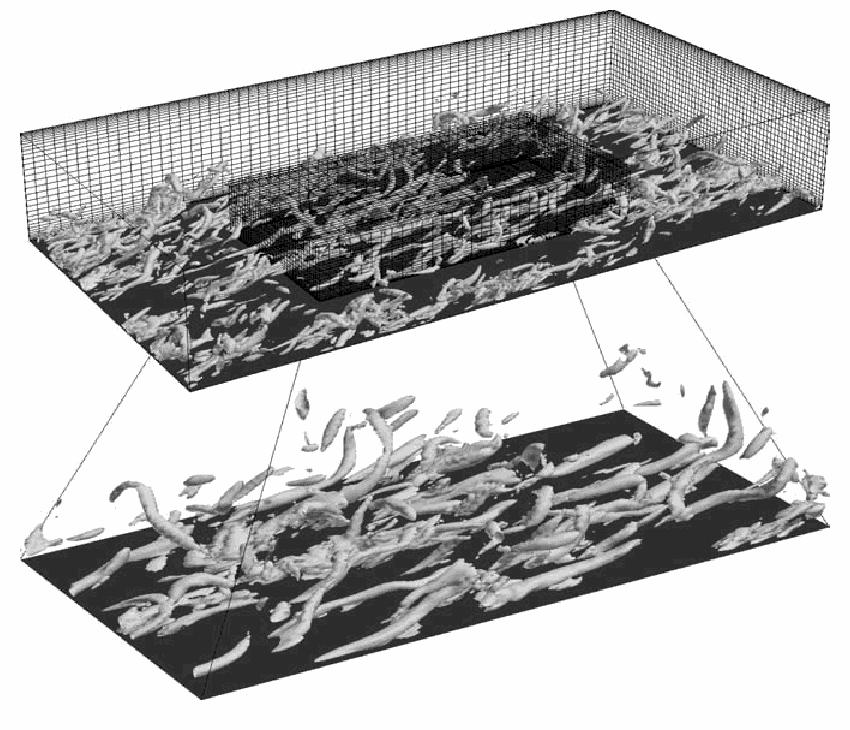
\includegraphics[width=0.78\textwidth]{figures/appendix03-figure01.png}
\caption{无控制通道流的边界层中相干结构的形成.}
\label{fig:app3-uncontrolled-channel-coherent-structures}
\end{figure}

\paragraph{流动控制.}
特别是在 20 世纪 90 年代, 流动控制方面形成了一定规模的研究活动; 人们研究了不可压缩黏性流和无黏流.

考虑形式为 \eqref{eq:app3-incompressible-nse-components}--\eqref{eq:app3-no-slip-boundary} 的 NSE, 但在 \eqref{eq:app3-no-slip-boundary} 中取 $u=g\not\equiv0$ 于 $\partial\Omega$, 并假设 $f$ 和 $g$ 可受控制. 我们希望以最佳方式选择 $f$ 和/或 $g$, 使 $u$ 和/或 $p$ 达到某些目标. Lions (1971)发展了偏微分方程控制的数学理论. 对 NS 方程, 最近研究了两类问题:
\begin{enumerate}
\item 湍流的最优控制与鲁棒控制;
\item 可控性, 包括 NS 方程和 Euler 方程.
\end{enumerate}
第二类问题是理论性的, 即数学问题; 第一类问题兼有理论性和计算性.

\hypertarget{appendix-03-page-377}{}
\begin{figure}[htbp]
\centering
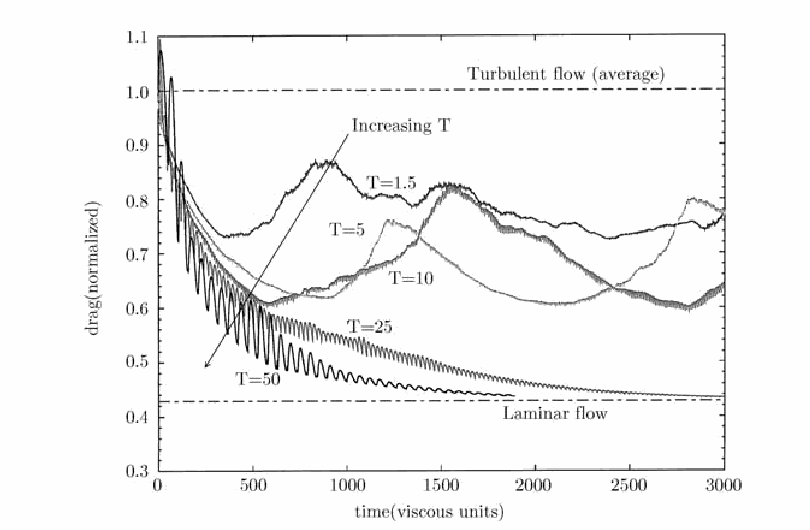
\includegraphics[width=0.72\textwidth]{figures/appendix03-figure02.png}
\caption{受控流中, 不同参数 $T$ 取值对应的阻力随时间演化.}
\label{fig:app3-controlled-flow-drag}
\end{figure}

对第一类问题, 最优控制的目标是减小由适当量度衡量的湍流, 例如旋度向量的 $L^2$ 范数或阻力; 这是一个变分法问题. 许多作者研究了该问题的不同形式, 见例如 M. Gunzburger (1989)主编的著作. 鲁棒控制是存在不利扰动时的控制问题, 见 Bewley, Moin and Temam (1997); 关于大量控制计算文献, 另见其中参考文献.

可控性问题是如何通过作用于控制量, 把流动引向某个期望状态. 控制量可以只是在 $\Omega$ 一部分上的 $f$, 或只是在 $\partial\Omega$ 一部分上的 $g$. 该问题与唯一延拓结果, 如 Mizohata (1958), Carleman 不等式, 以及当 $f$, $g$ 和可能的 $u_0$ 在适当集合中变化时像集 $\{u(T)\}$ 的刻画有关. 最初的结果, 问题描述和猜想见 Lions (1988, 1990). Fursikov (1995), Fursikov and Imanuvilov (1994, 1996a,b)在一系列论文中证明, 对线性化方程和 NS 方程, 通过 $f$ 或 $g$ 可得到局部精确可控性. Coron and Fursikov (1996)证明无边界流形上二维 Navier--Stokes 方程的整体精确可控性. Coron (1996a)得到带 Dirichlet 边界条件的二维 NSE 可控性的一些部分结果. Coron (1996b)证明二维不可压缩 Euler 方程的近似边界可控性, 即通过 $g$ 控制, 以及分布可控性, 即通过 $f$ 控制.

图 \ref{fig:app3-uncontrolled-channel-coherent-structures} 显示通道流边界层中涡旋的出现, 这是无控制流的数值模拟. 图 \ref{fig:app3-controlled-flow-drag} 显示受控通道流中阻力降低到几乎绝对最小值, 即层流的阻力; 该图取自 Bewley, Moin and Temam (1997). 相应计算涉及 1700 万个空间模态.

\clearpage
\section*{附录 III 参考文献}
\label{sec:app3-bibliography}

这份扩展参考文献包含许多未在附录 III 或本书中引用的文献. 其中一些文献可能与第一份参考文献表中的条目重复. 为严格保留作者姓名, 文献题名, 卷期, 页码和原始语言, 以下书目条目按原书逐页保留.

\hypertarget{appendix-03-page-378}{}
\noindent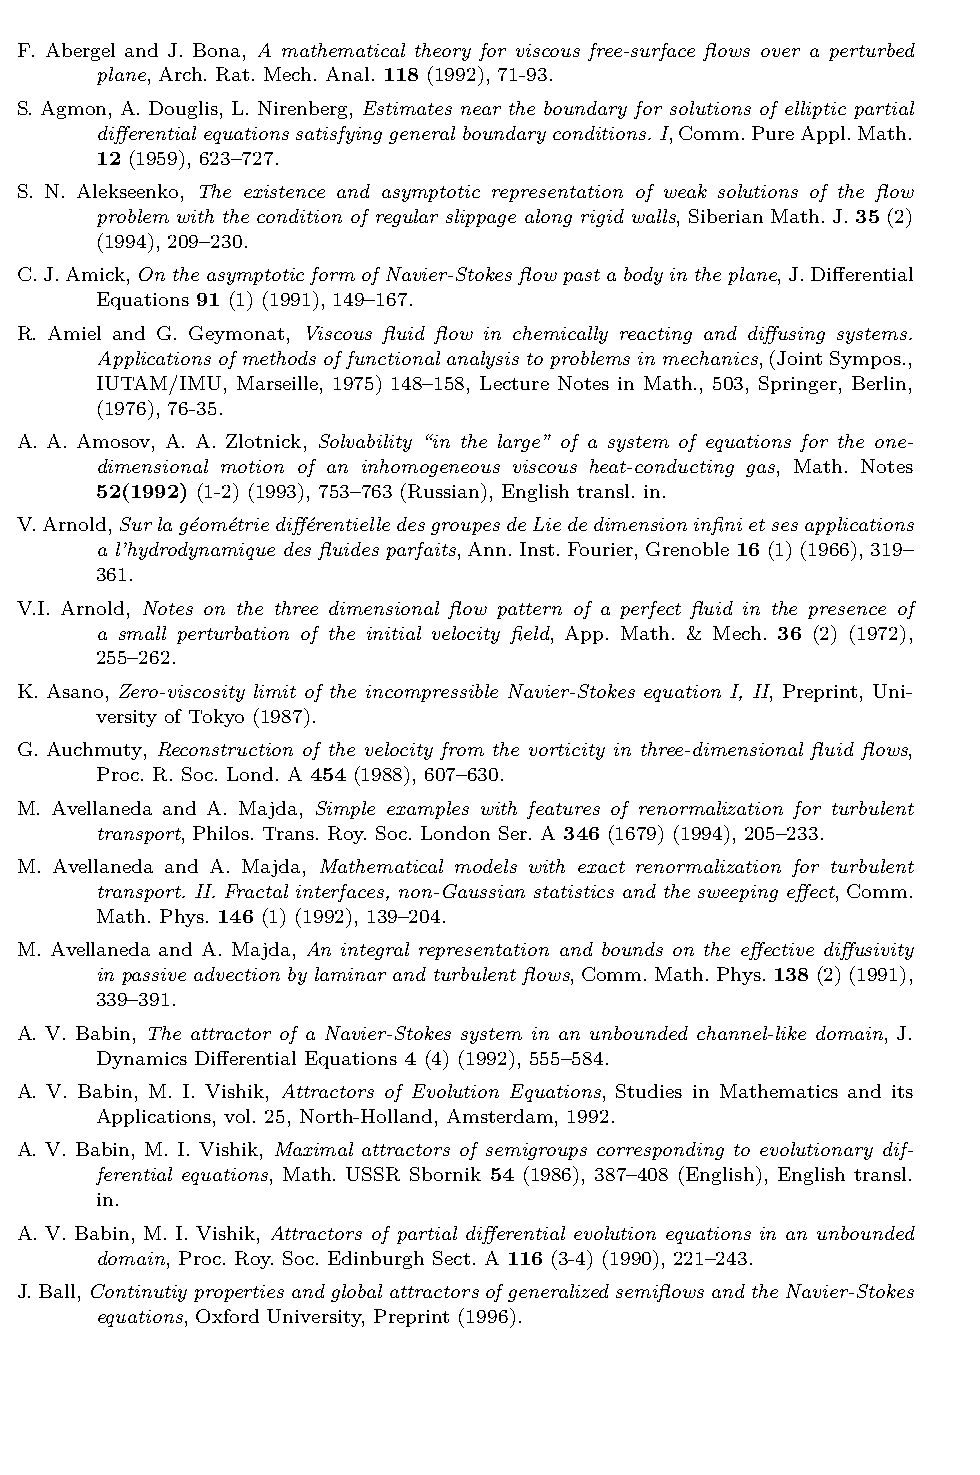
\includegraphics[width=\textwidth,height=0.84\textheight,keepaspectratio]{figures/appendix03-bibliography-378.png}
\clearpage
\hypertarget{appendix-03-page-379}{}
\noindent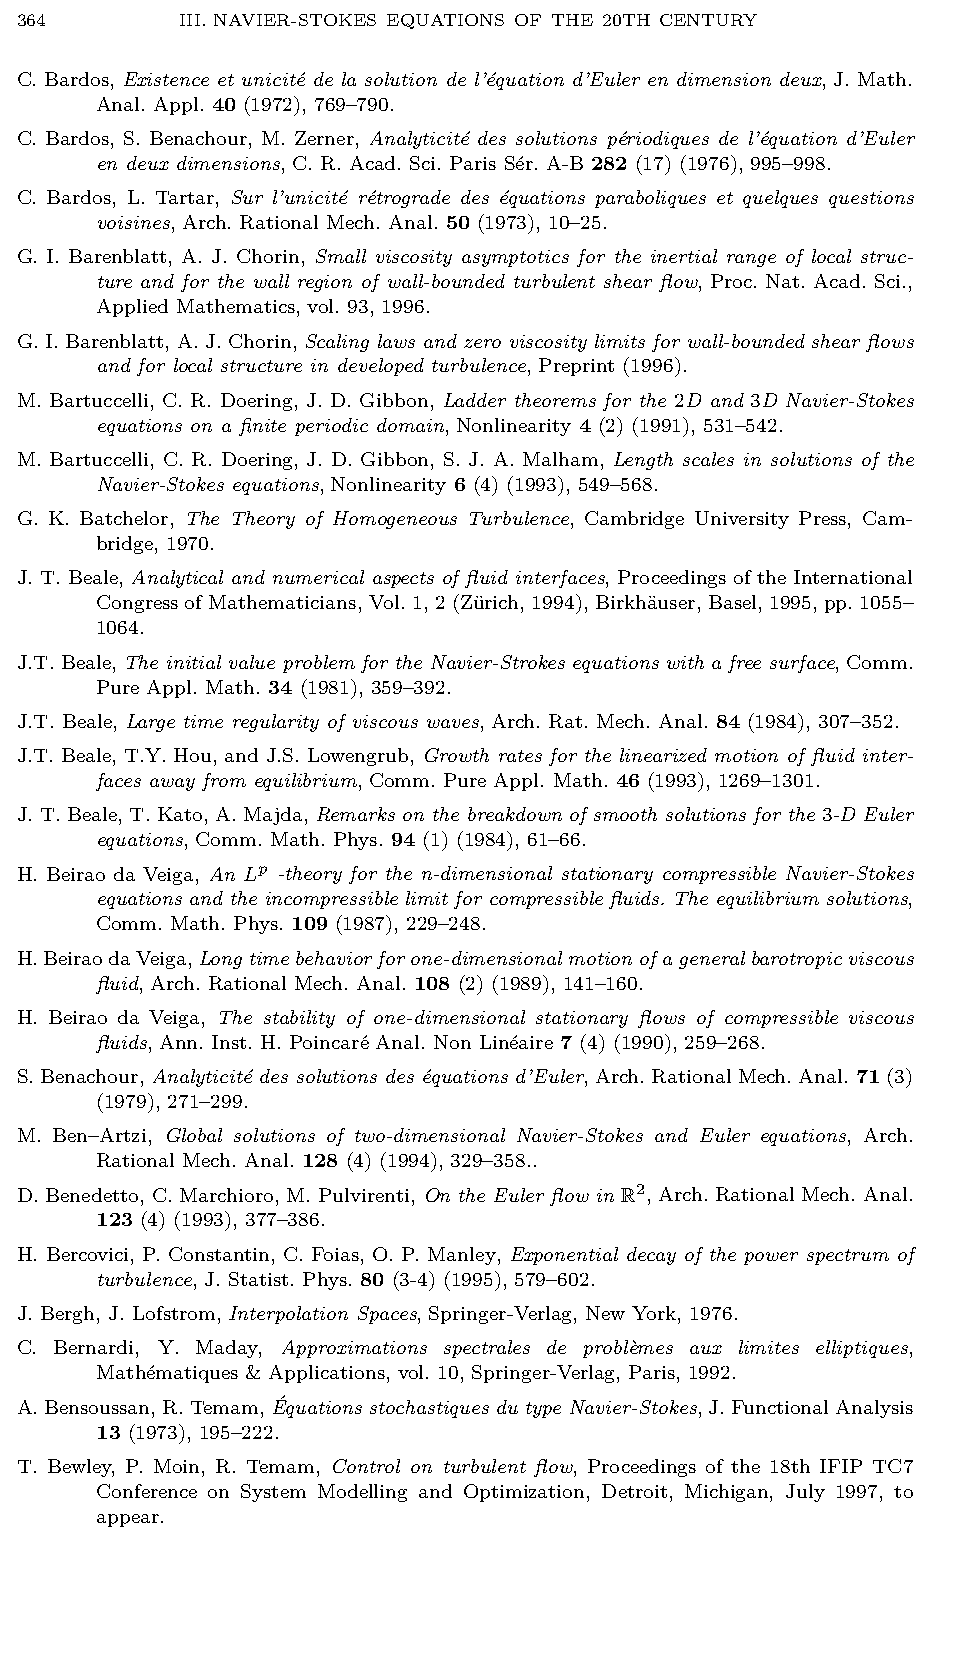
\includegraphics[width=\textwidth,height=0.91\textheight,keepaspectratio]{figures/appendix03-bibliography-379.png}
\clearpage
\hypertarget{appendix-03-page-380}{}
\noindent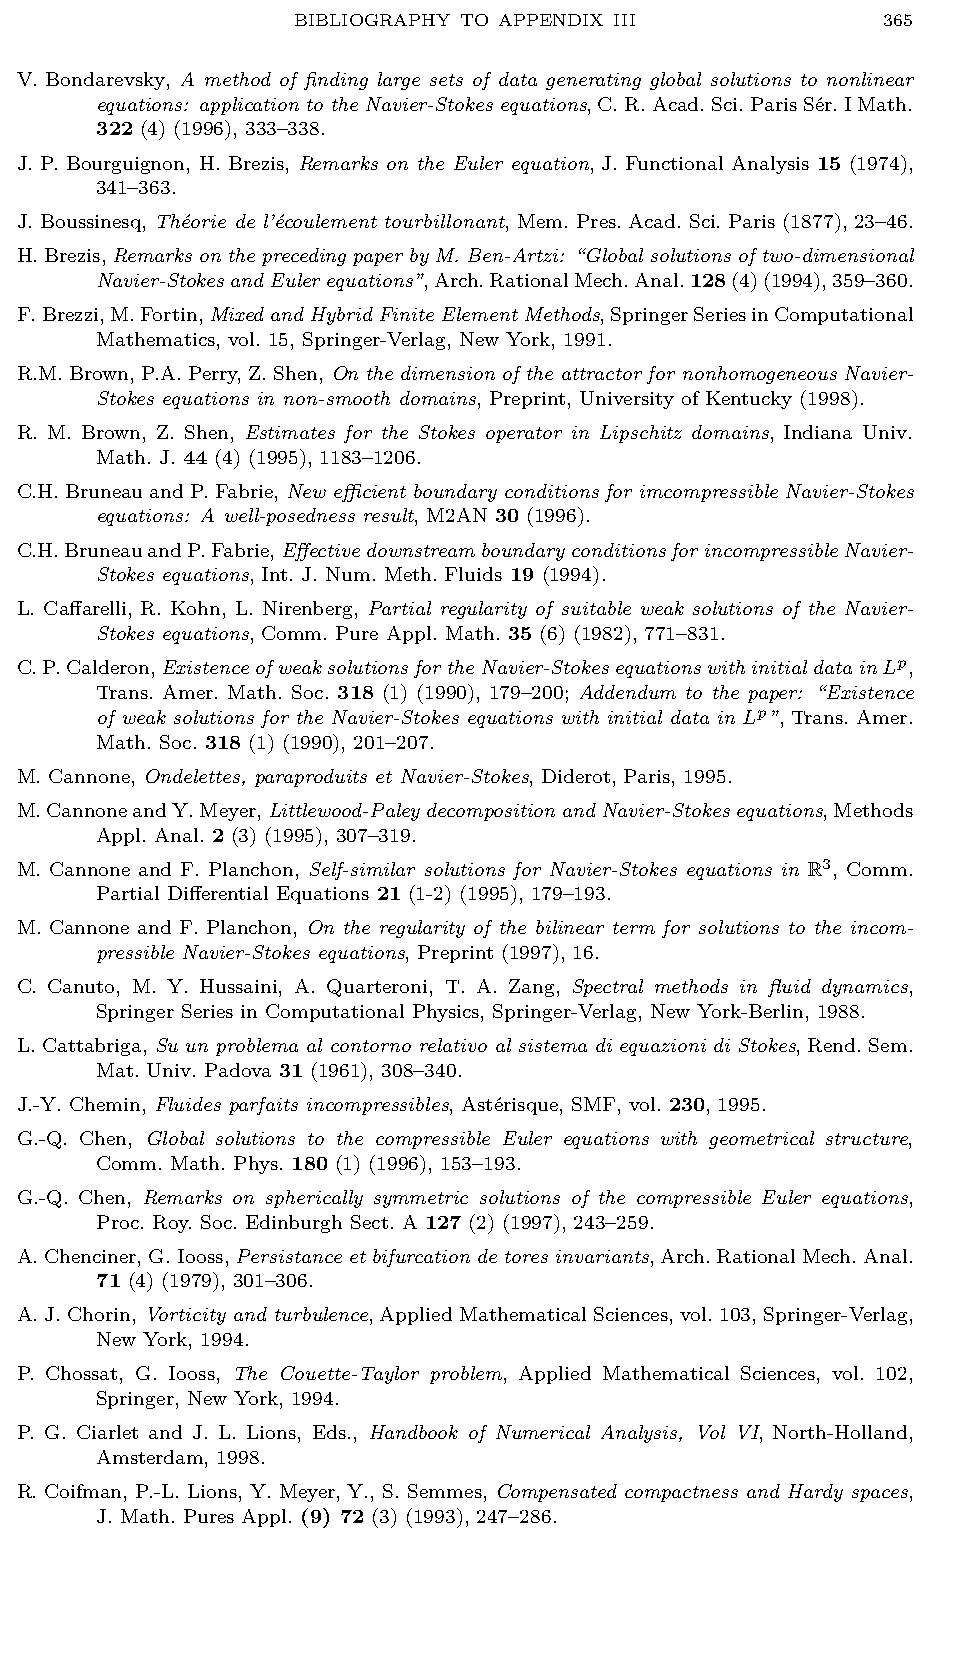
\includegraphics[width=\textwidth,height=0.91\textheight,keepaspectratio]{figures/appendix03-bibliography-380.png}
\clearpage
\hypertarget{appendix-03-page-381}{}
\noindent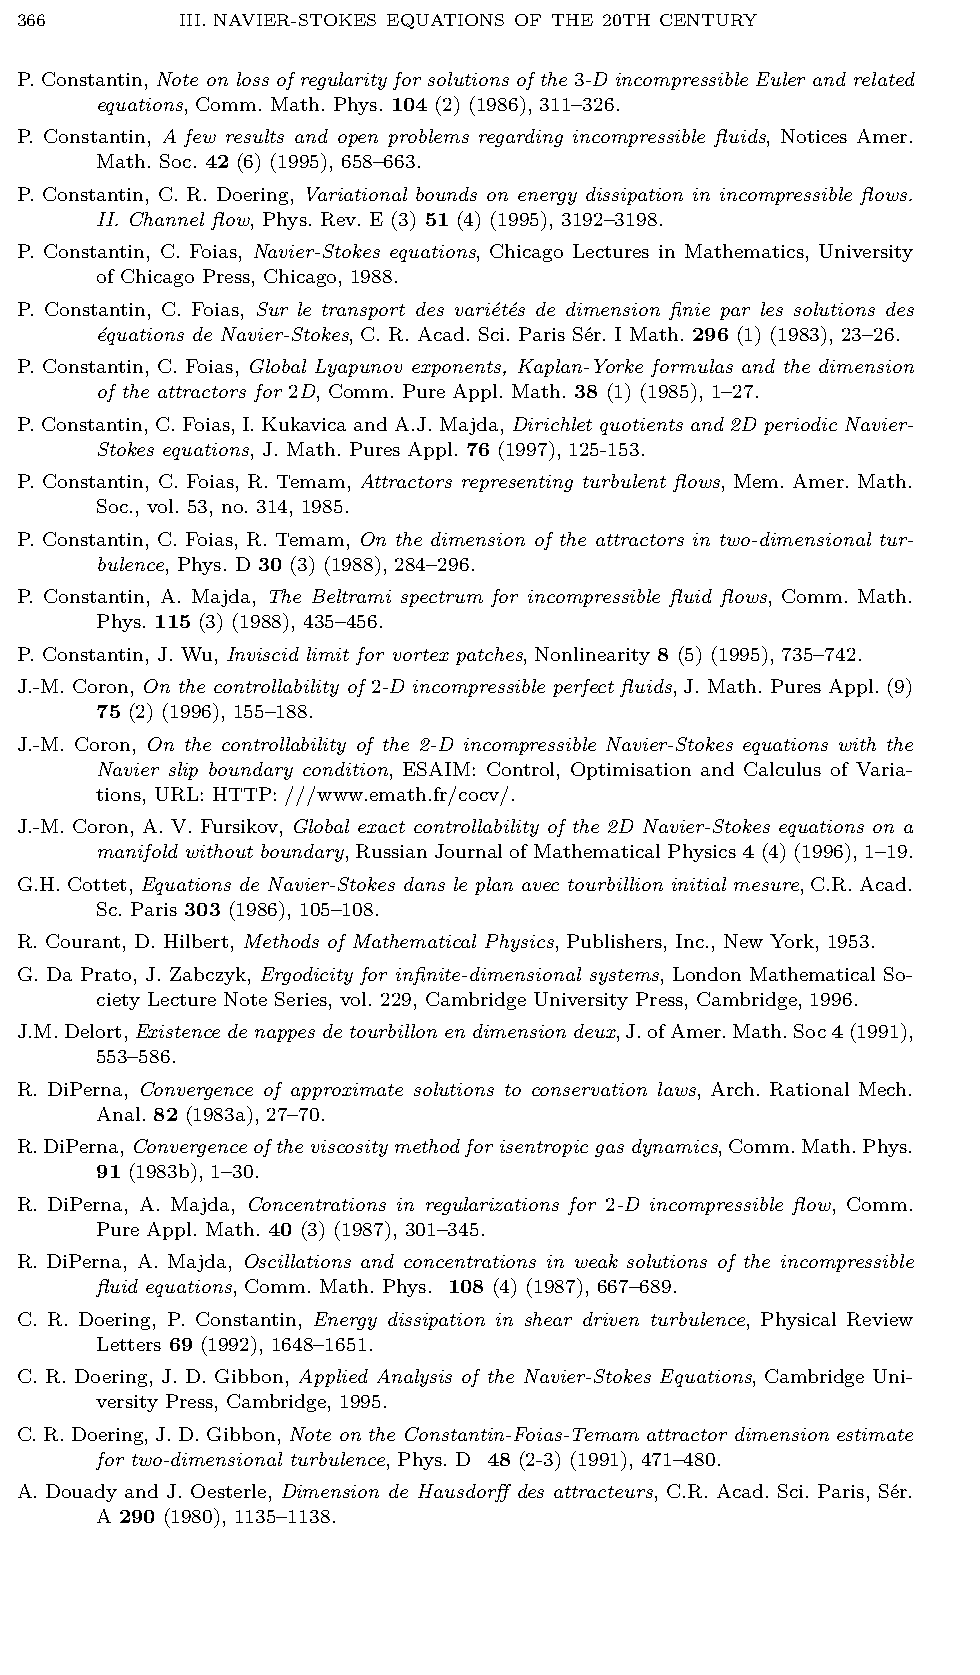
\includegraphics[width=\textwidth,height=0.91\textheight,keepaspectratio]{figures/appendix03-bibliography-381.png}
\clearpage
\hypertarget{appendix-03-page-382}{}
\noindent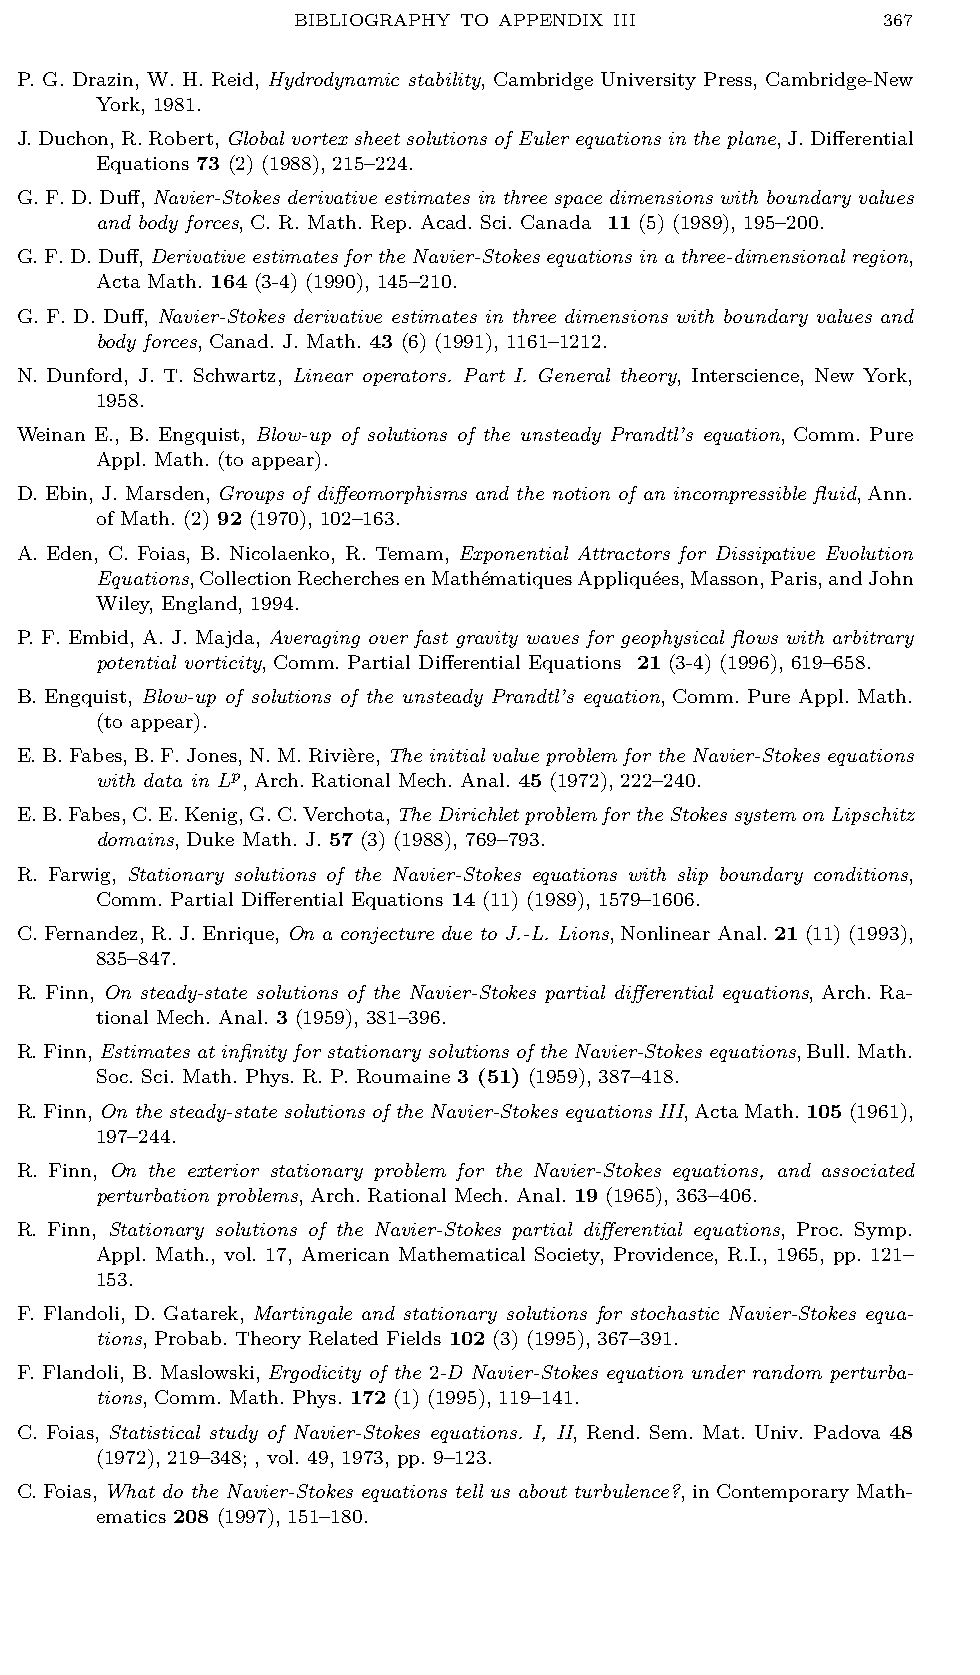
\includegraphics[width=\textwidth,height=0.91\textheight,keepaspectratio]{figures/appendix03-bibliography-382.png}
\clearpage
\hypertarget{appendix-03-page-383}{}
\noindent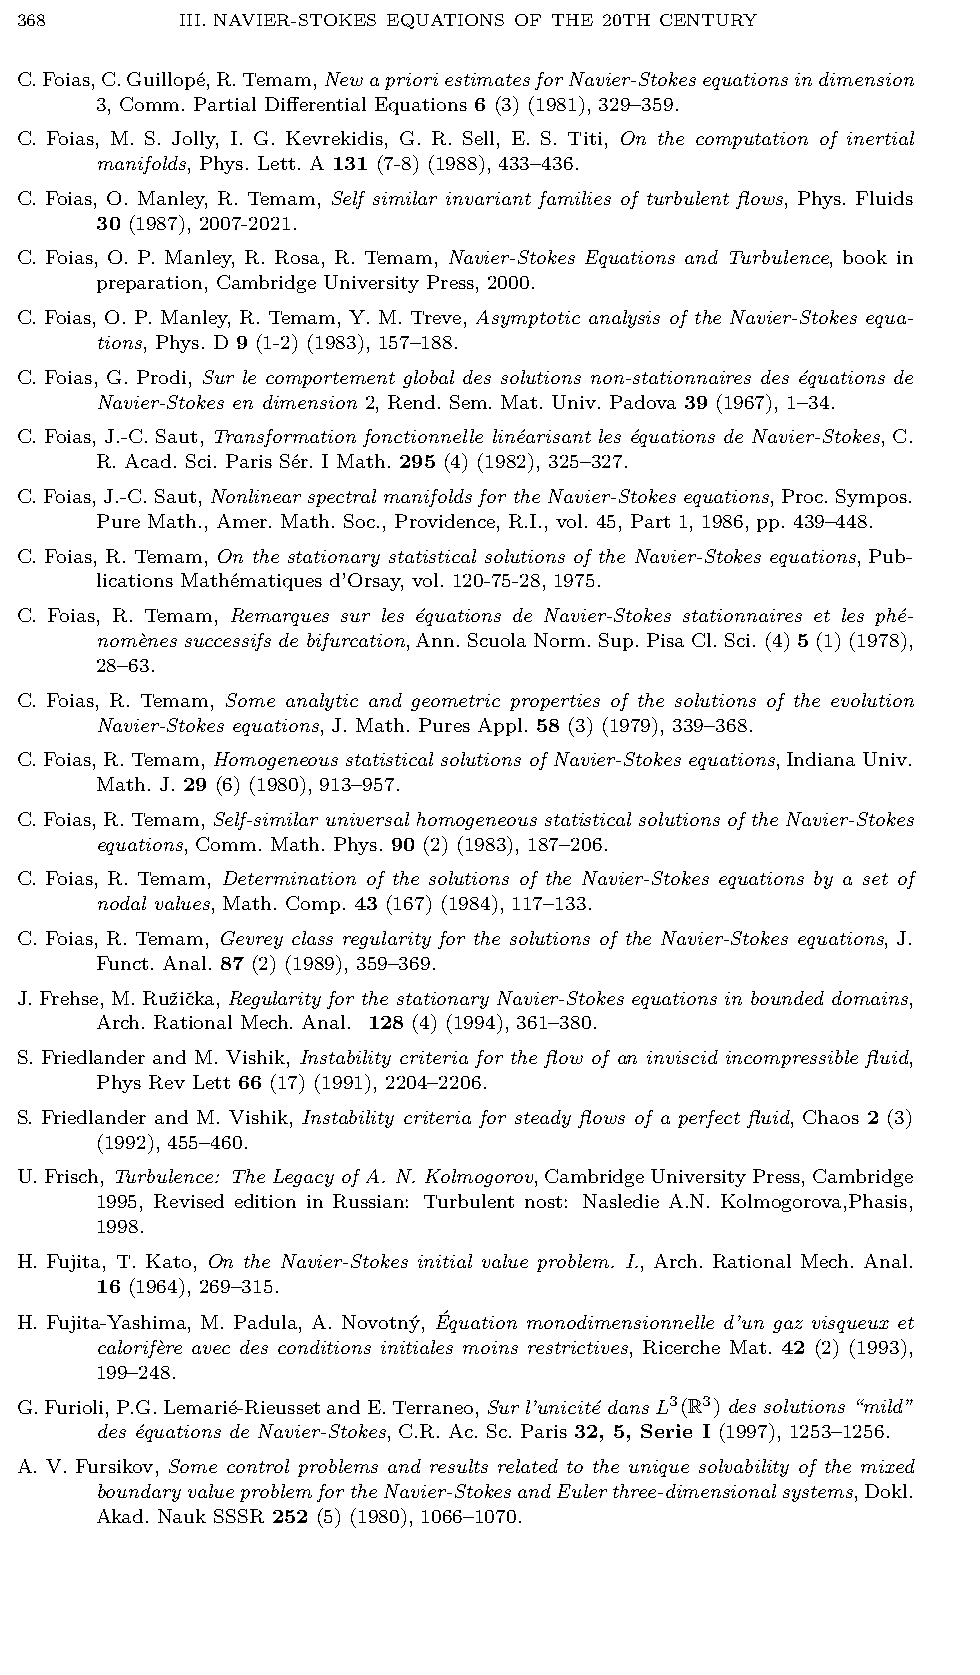
\includegraphics[width=\textwidth,height=0.91\textheight,keepaspectratio]{figures/appendix03-bibliography-383.png}
\clearpage
\hypertarget{appendix-03-page-384}{}
\noindent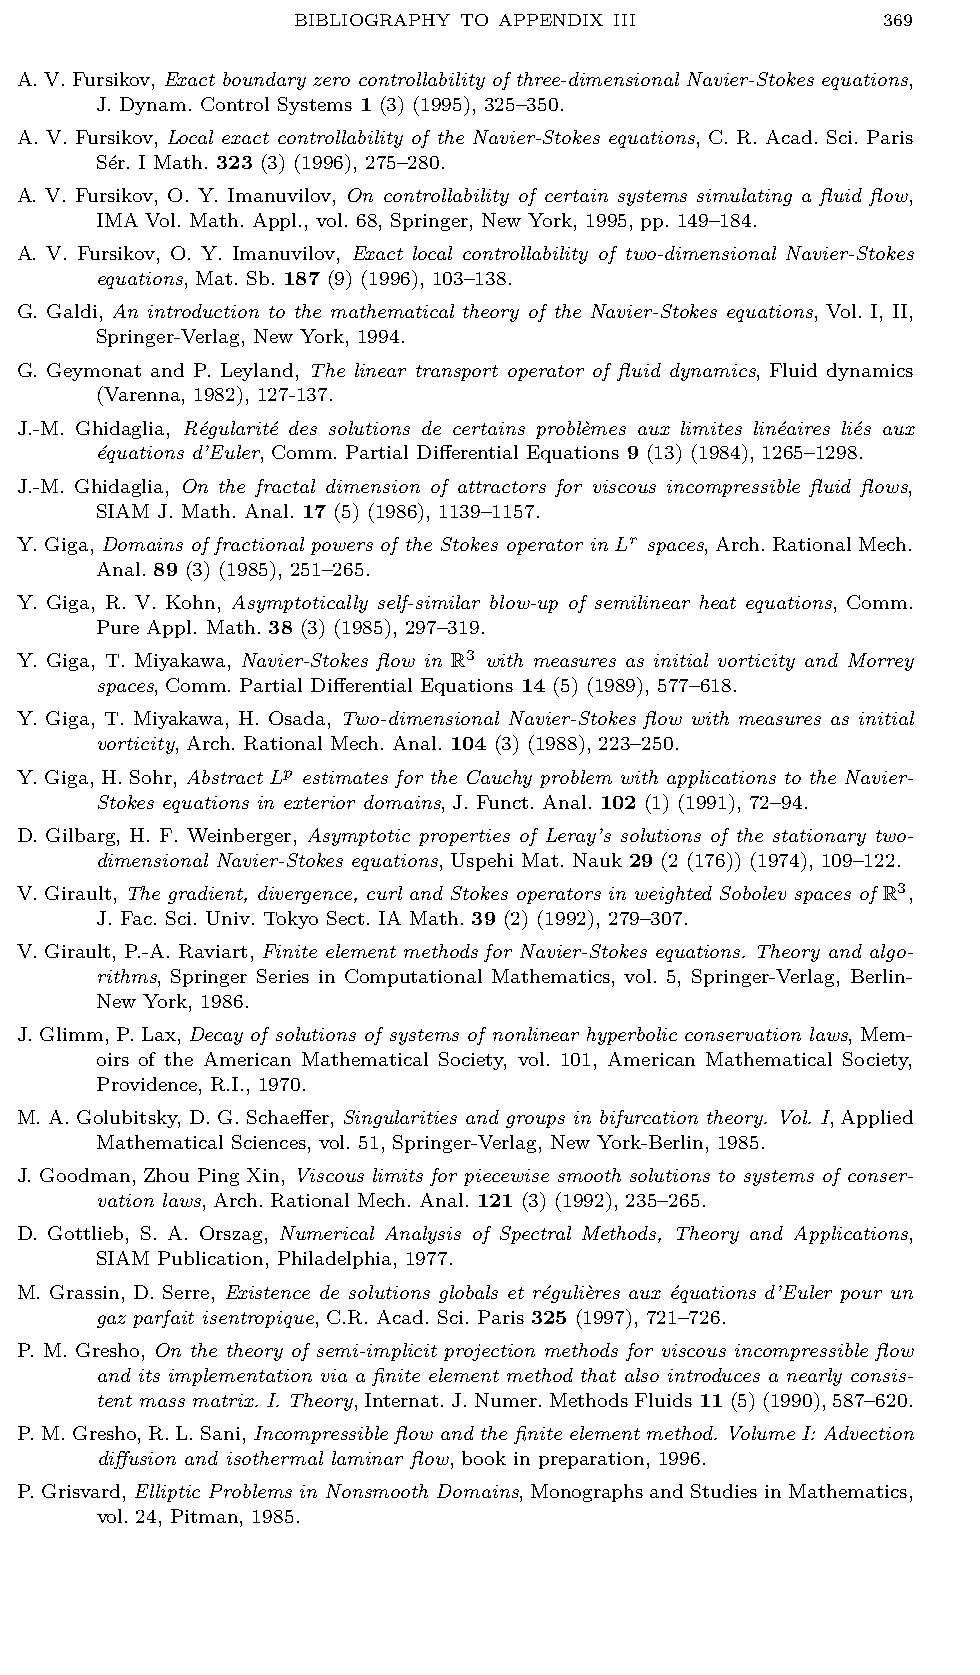
\includegraphics[width=\textwidth,height=0.91\textheight,keepaspectratio]{figures/appendix03-bibliography-384.png}
\clearpage
\hypertarget{appendix-03-page-385}{}
\noindent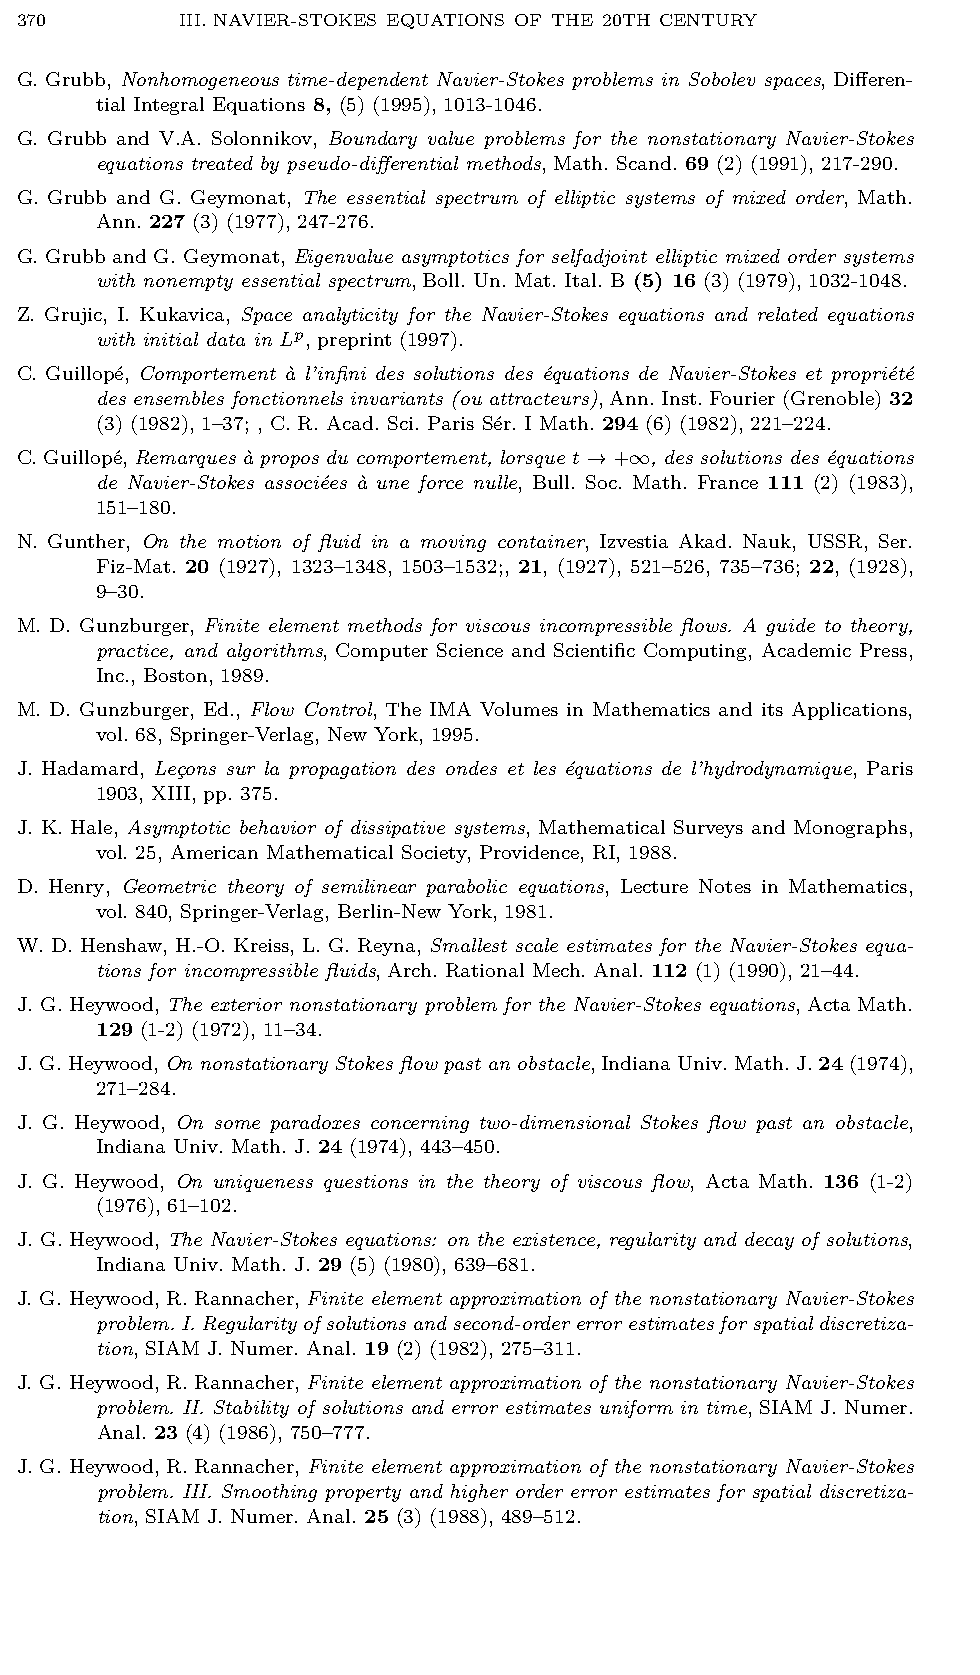
\includegraphics[width=\textwidth,height=0.91\textheight,keepaspectratio]{figures/appendix03-bibliography-385.png}
\clearpage
\hypertarget{appendix-03-page-386}{}
\noindent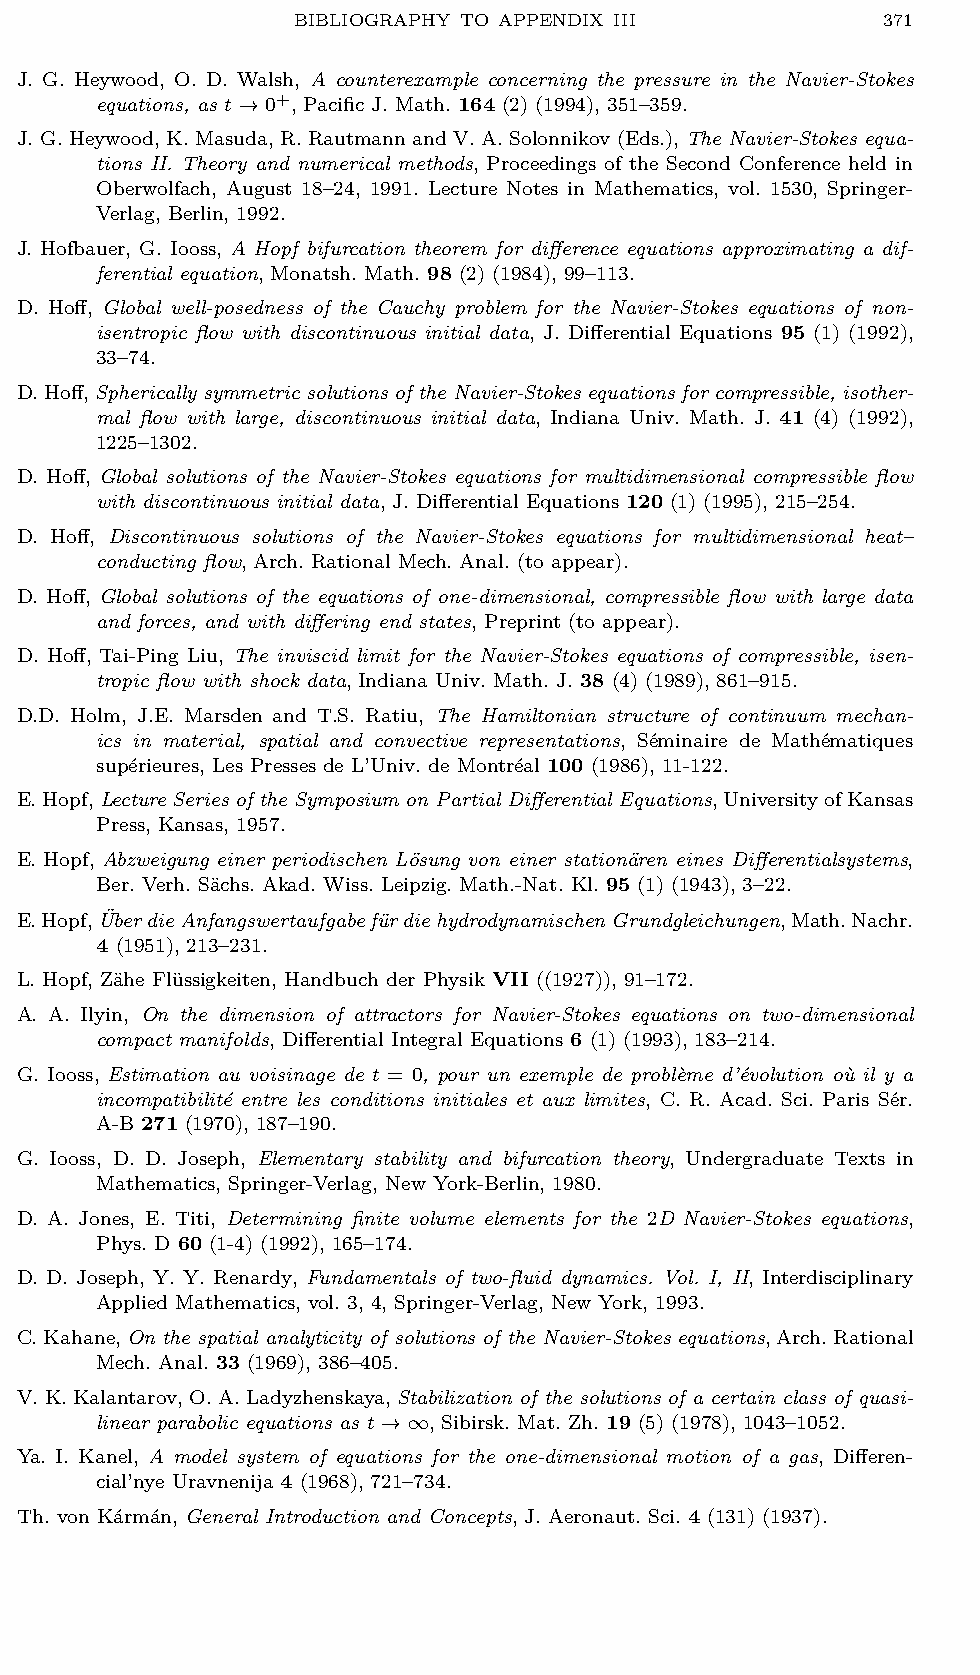
\includegraphics[width=\textwidth,height=0.91\textheight,keepaspectratio]{figures/appendix03-bibliography-386.png}
\clearpage
\hypertarget{appendix-03-page-387}{}
\noindent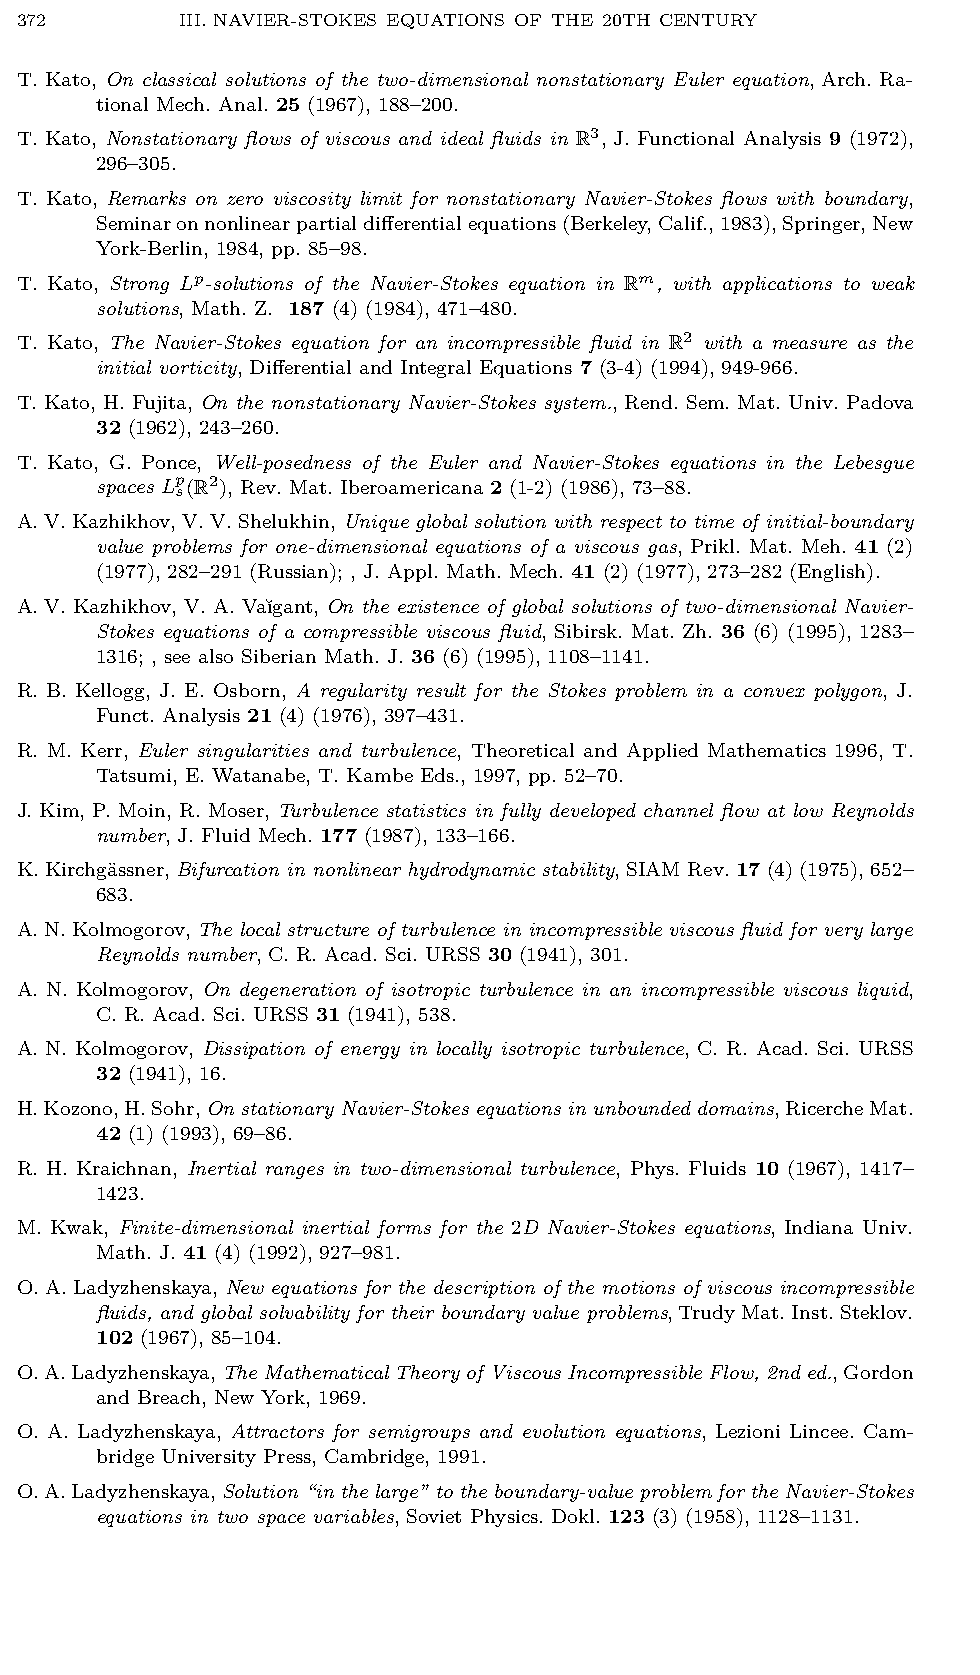
\includegraphics[width=\textwidth,height=0.91\textheight,keepaspectratio]{figures/appendix03-bibliography-387.png}
\clearpage
\hypertarget{appendix-03-page-388}{}
\noindent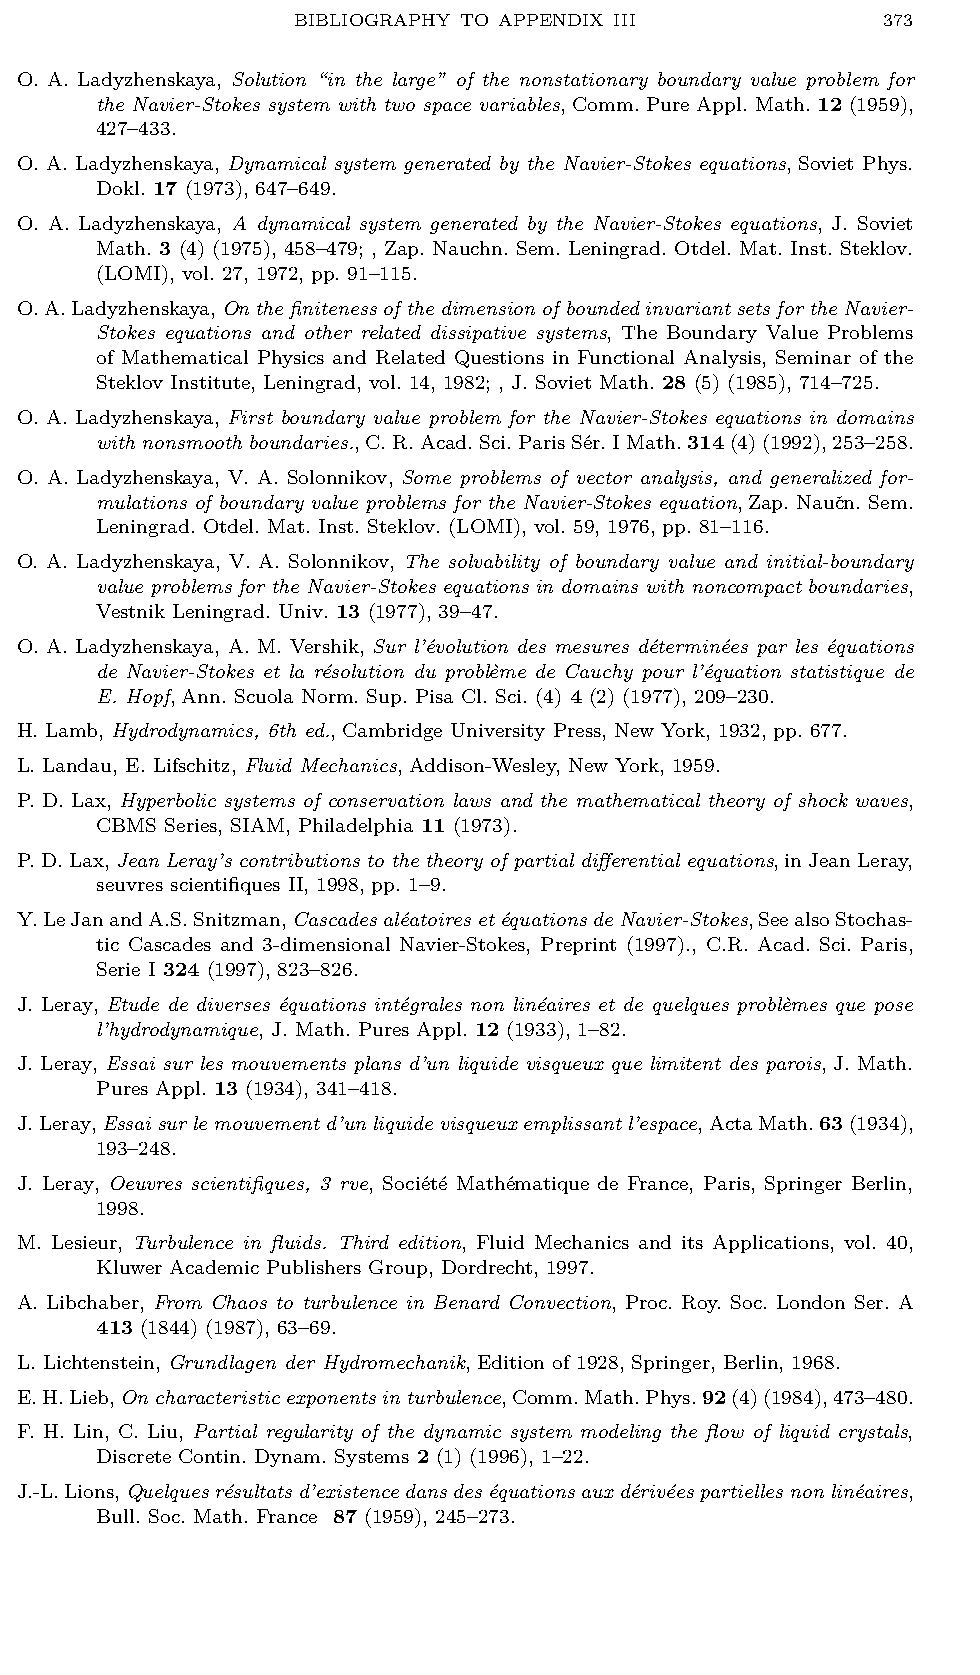
\includegraphics[width=\textwidth,height=0.91\textheight,keepaspectratio]{figures/appendix03-bibliography-388.png}
\clearpage
\hypertarget{appendix-03-page-389}{}
\noindent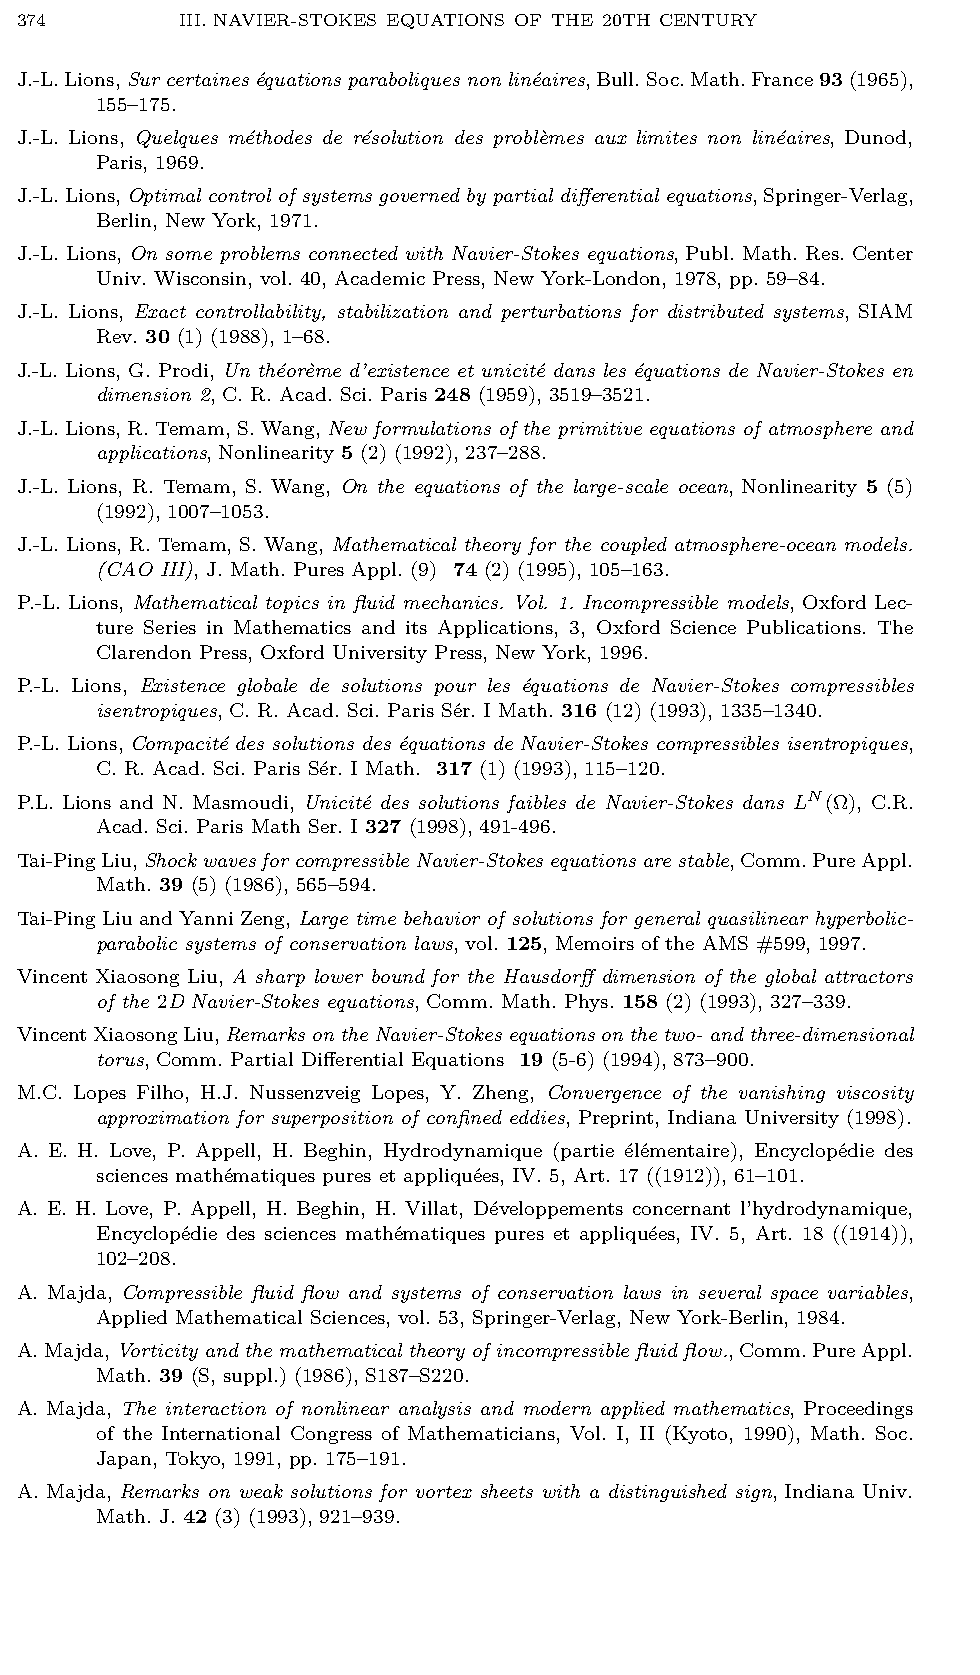
\includegraphics[width=\textwidth,height=0.91\textheight,keepaspectratio]{figures/appendix03-bibliography-389.png}
\clearpage
\hypertarget{appendix-03-page-390}{}
\noindent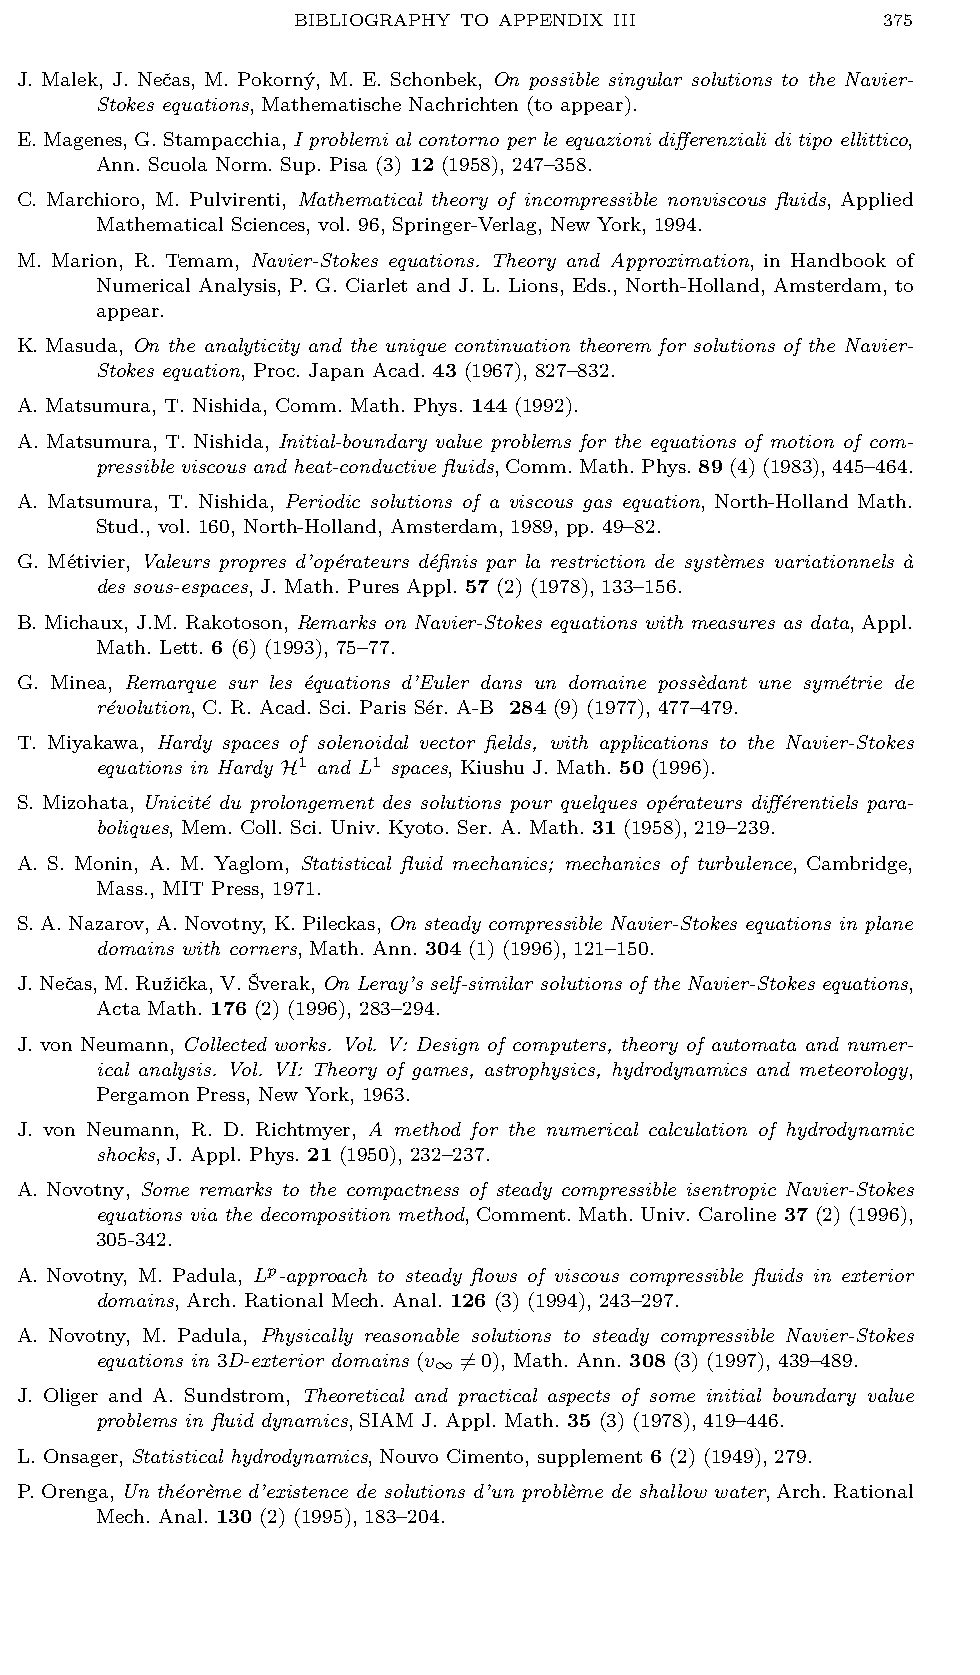
\includegraphics[width=\textwidth,height=0.91\textheight,keepaspectratio]{figures/appendix03-bibliography-390.png}
\clearpage
\hypertarget{appendix-03-page-391}{}
\noindent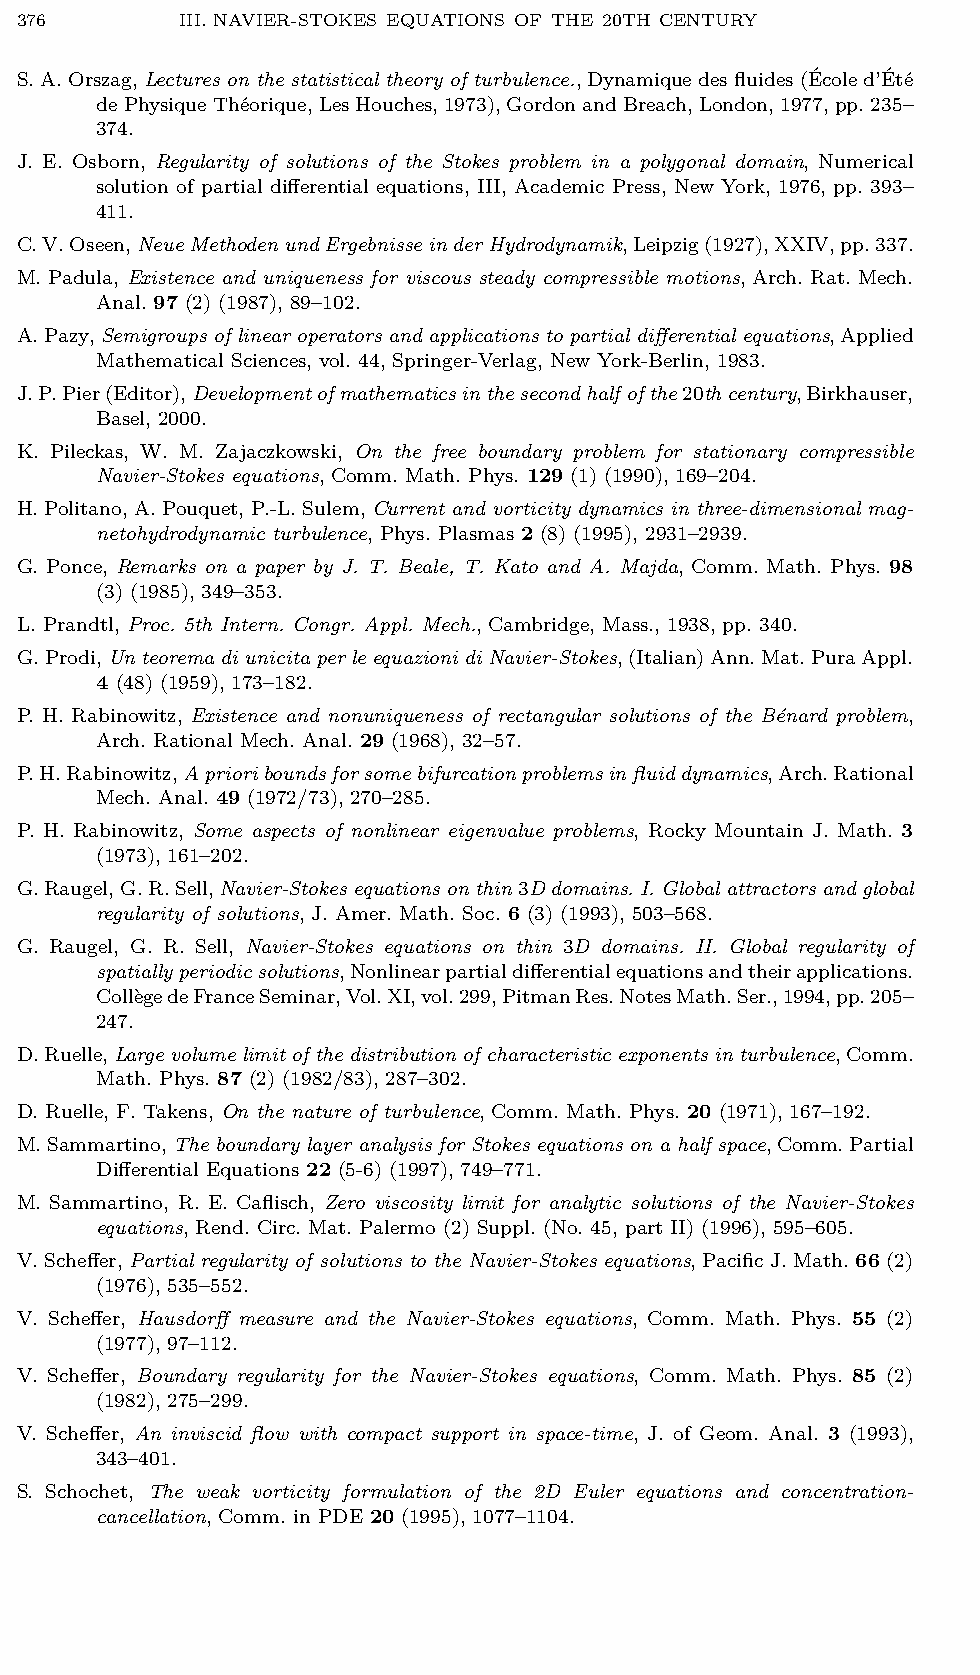
\includegraphics[width=\textwidth,height=0.91\textheight,keepaspectratio]{figures/appendix03-bibliography-391.png}
\clearpage
\hypertarget{appendix-03-page-392}{}
\noindent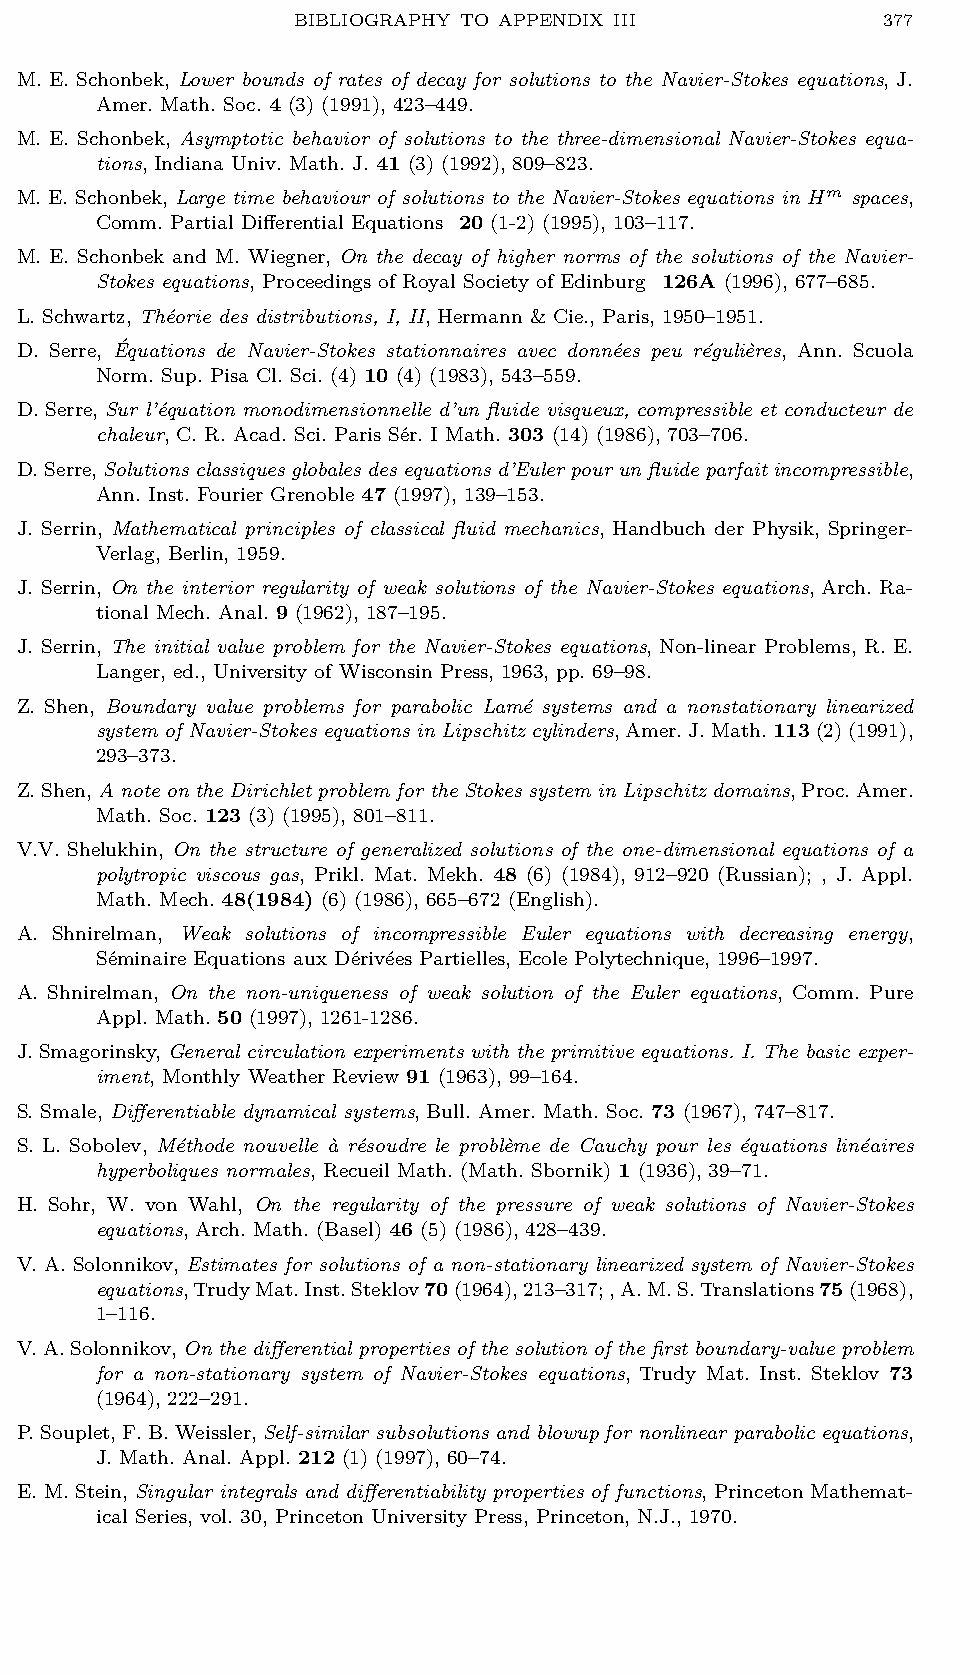
\includegraphics[width=\textwidth,height=0.91\textheight,keepaspectratio]{figures/appendix03-bibliography-392.png}
\clearpage
\hypertarget{appendix-03-page-393}{}
\noindent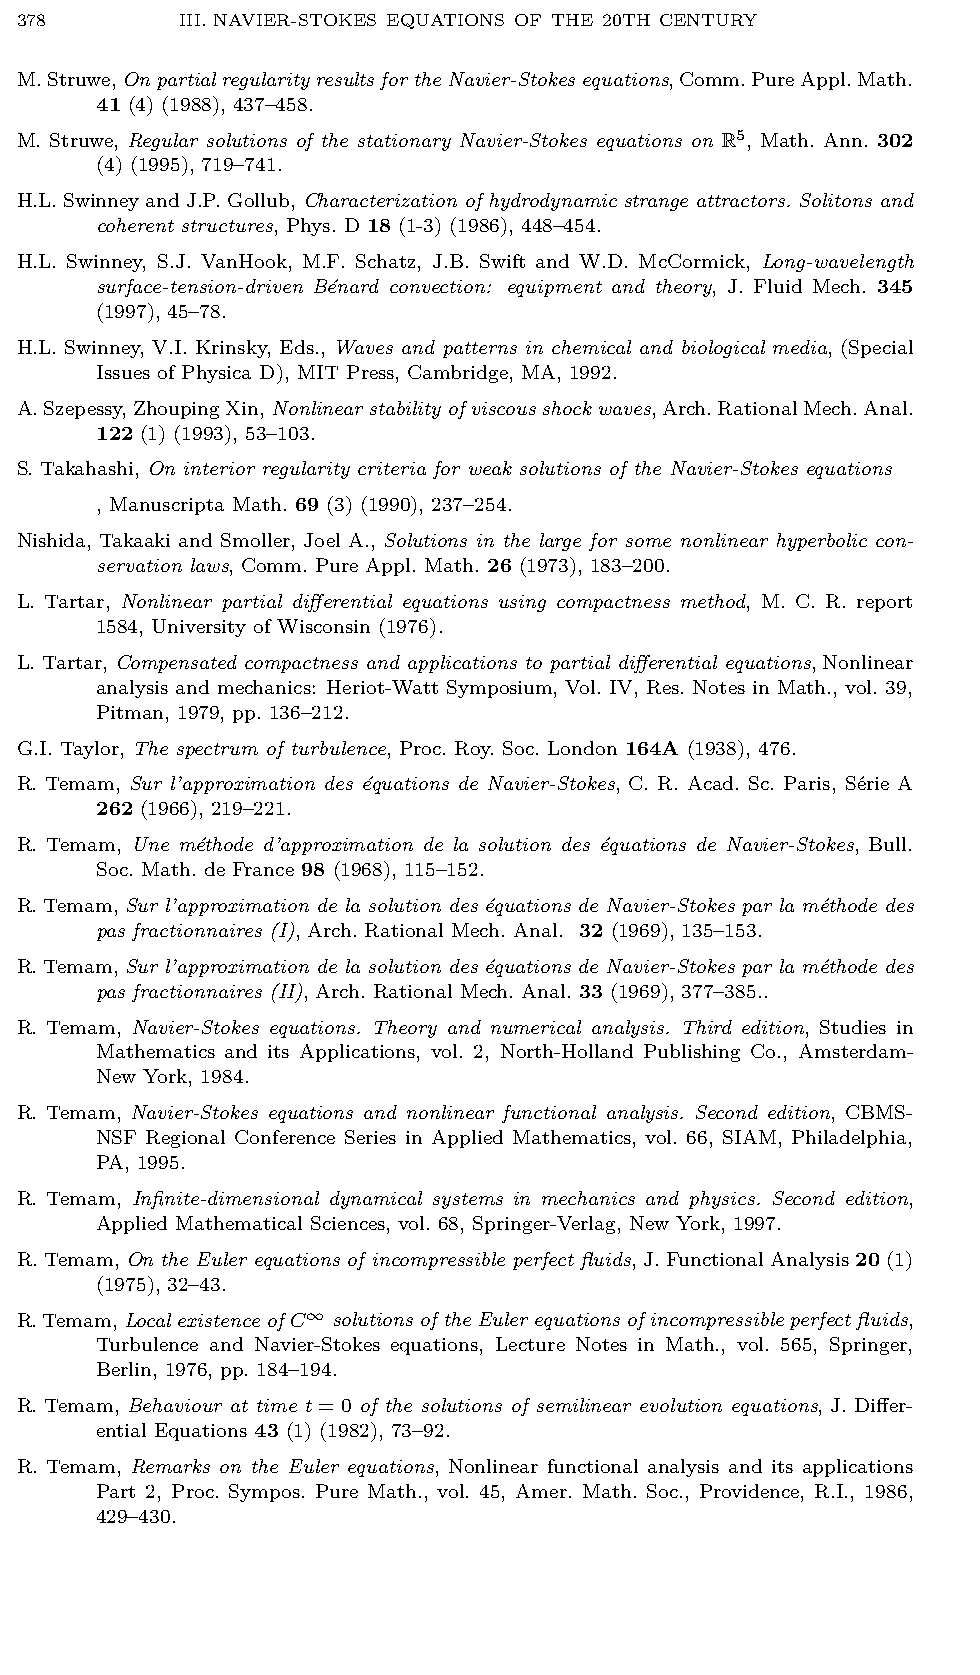
\includegraphics[width=\textwidth,height=0.91\textheight,keepaspectratio]{figures/appendix03-bibliography-393.png}
\clearpage
\hypertarget{appendix-03-page-394}{}
\noindent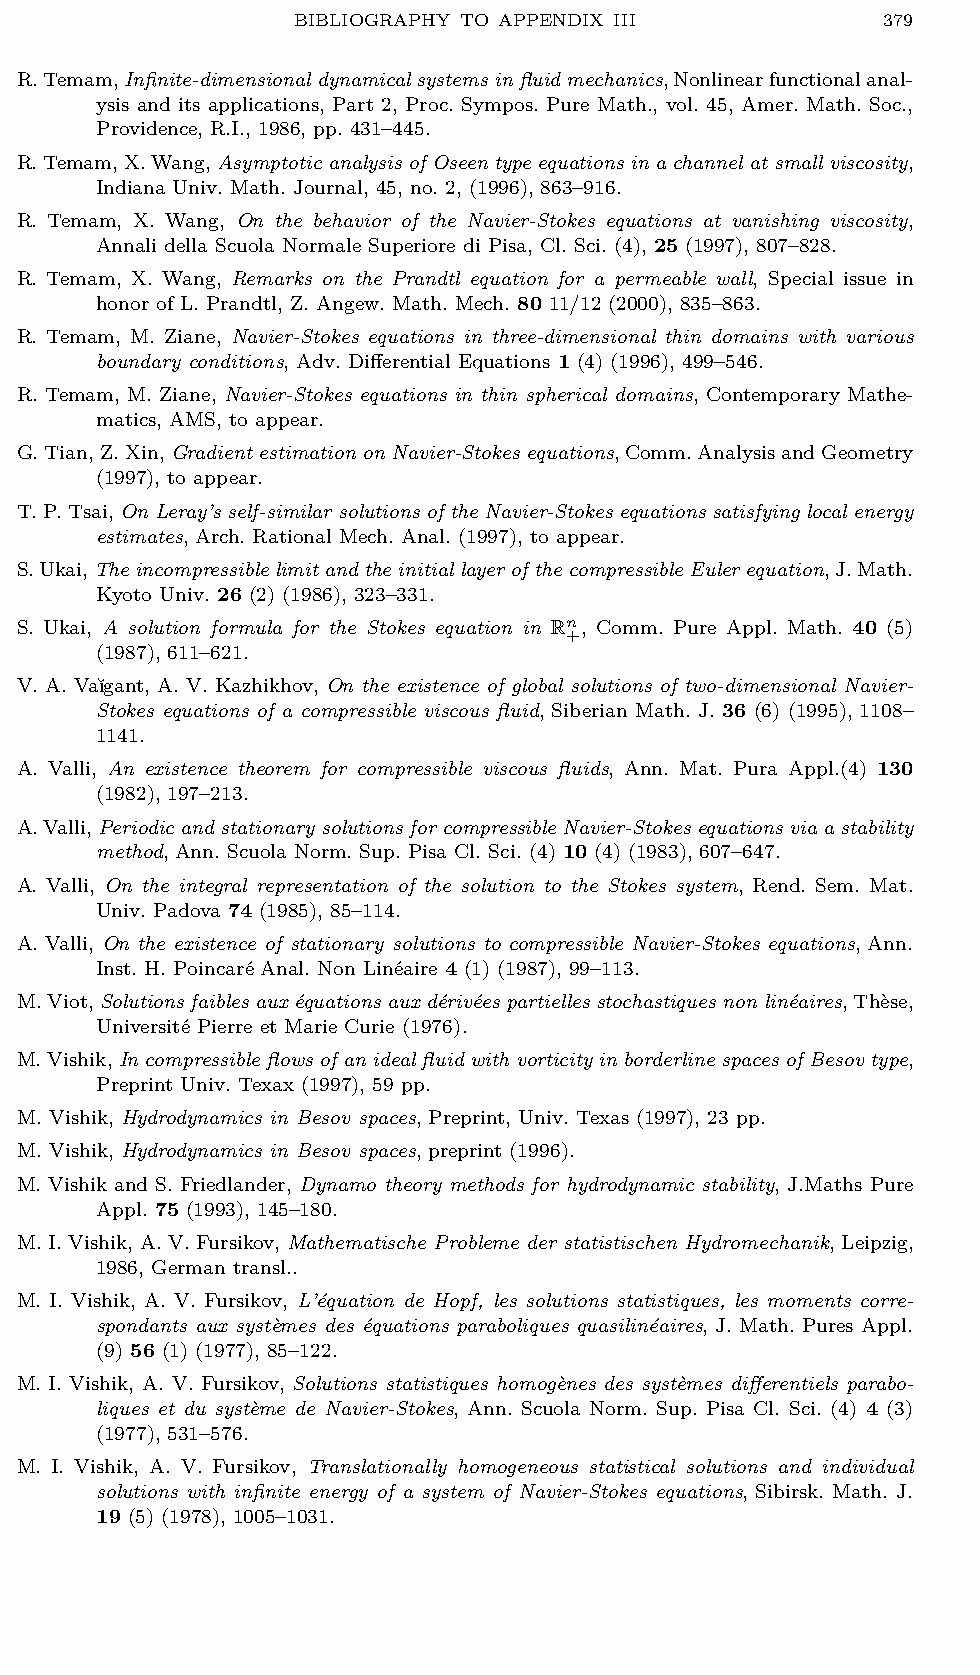
\includegraphics[width=\textwidth,height=0.91\textheight,keepaspectratio]{figures/appendix03-bibliography-394.png}
\clearpage
\hypertarget{appendix-03-page-395}{}
\noindent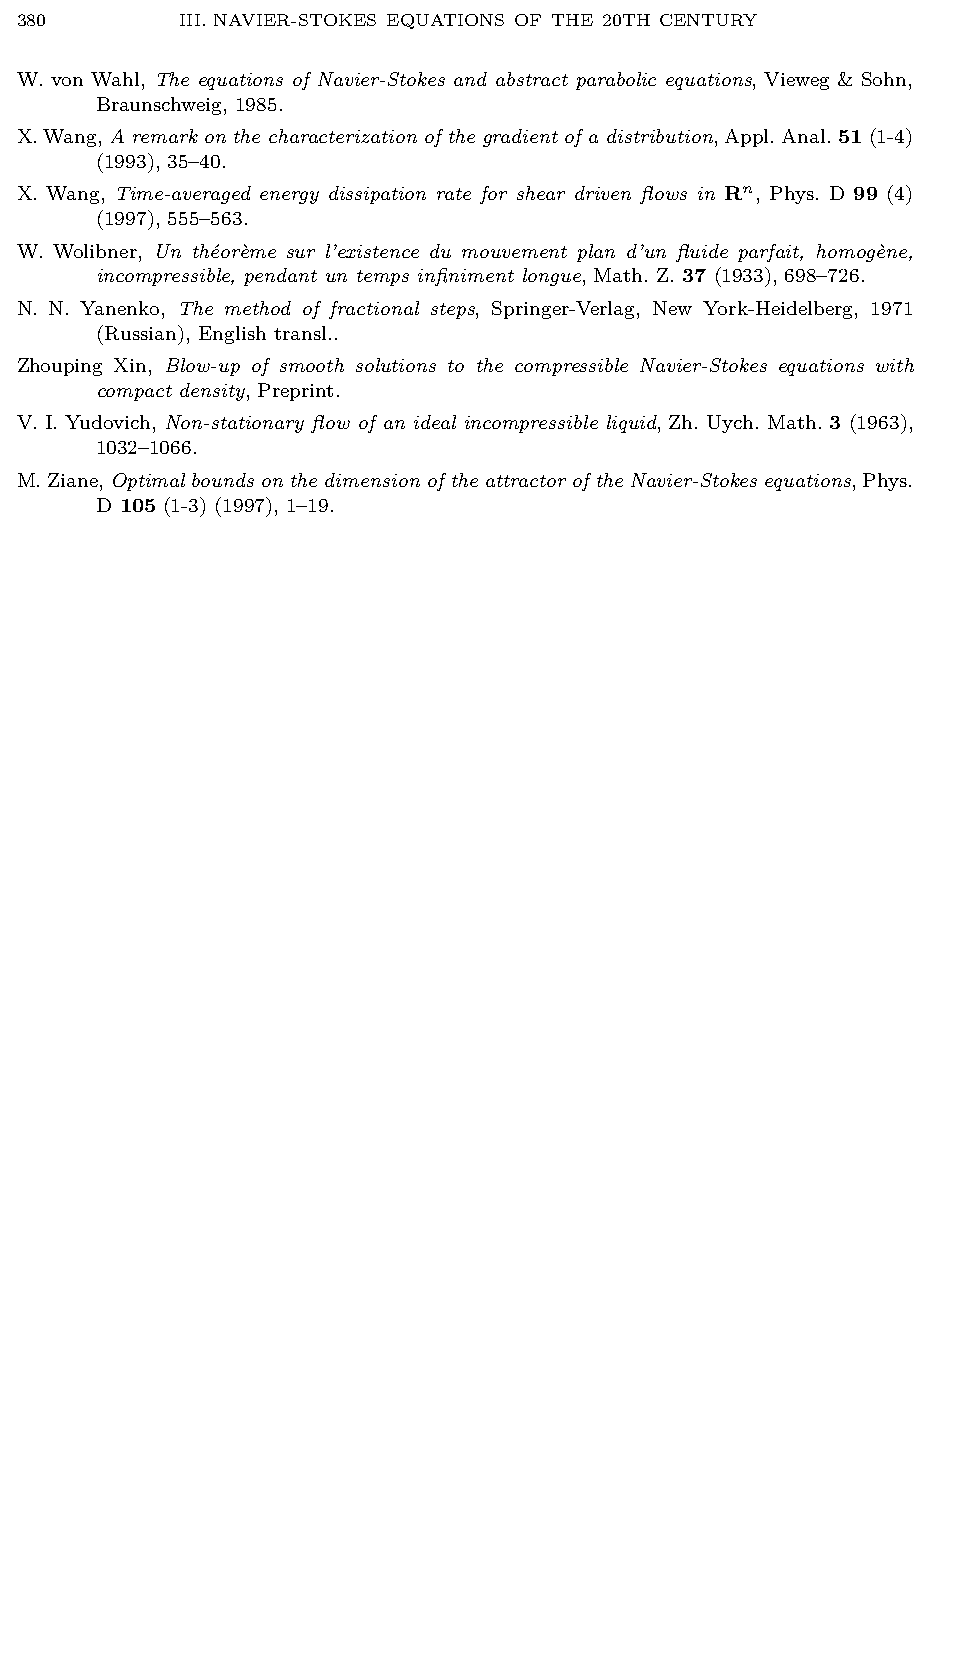
\includegraphics[width=\textwidth,height=0.91\textheight,keepaspectratio]{figures/appendix03-bibliography-395.png}

\renewcommand{\theequation}{\thesection.\arabic{equation}}
